\documentclass{article}
\usepackage[utf8]{inputenc}
\usepackage{graphicx}
\usepackage{mathtools}
\linespread{1.1}



\usepackage{tikz}
\usetikzlibrary{positioning}

\usepackage{amsmath,amssymb}
\usepackage{hyperref}
\usepackage{xcolor}
\usepackage{listings}
\usepackage{xcolor}
\usepackage{graphicx}
\graphicspath{{./images/}}
\usepackage{float}
\usepackage{subfig}
\usepackage{natbib}
\bibliographystyle{abbrvnat}
\setcitestyle{authoryear,open={(},close={)}}
\raggedbottom

\definecolor{codegreen}{rgb}{0,0.6,0}
\definecolor{codegray}{rgb}{0.5,0.5,0.5}
\definecolor{codepurple}{rgb}{0.58,0,0.82}
\definecolor{backcolour}{rgb}{0.95,0.95,0.92}
\definecolor{myyellow}{rgb}{0.7,0.4,0}


\lstdefinestyle{mystyle}{
    backgroundcolor=\color{backcolour},   
    commentstyle=\color{codegreen},
    keywordstyle=\color{magenta},
    numberstyle=\tiny\color{codegray},
    stringstyle=\color{codepurple},
    basicstyle=\ttfamily\footnotesize,
    breakatwhitespace=false,         
    breaklines=true,                 
    captionpos=b,                    
    keepspaces=true,                 
    numbers=left,                    
    numbersep=5pt,                  
    showspaces=false,                
    showstringspaces=false,
    showtabs=false,                  
    tabsize=2
}

\lstset{style=mystyle}


\DeclareRobustCommand{\bbone}{\text{\usefont{U}{bbold}{m}{n}1}}

\DeclareMathOperator{\EX}{\mathbb{E}}% expected value

\newcommand{\R}{\mathbb{R}} % Real numbers space


\renewcommand{\texttt}[1]{%
  \begingroup
  \ttfamily
  \begingroup\lccode`~=`/\lowercase{\endgroup\def~}{/\discretionary{}{}{}}%
  \begingroup\lccode`~=`[\lowercase{\endgroup\def~}{[\discretionary{}{}{}}%
  \begingroup\lccode`~=`.\lowercase{\endgroup\def~}{.\discretionary{}{}{}}%
  \catcode`/=\active\catcode`[=\active\catcode`.=\active
  \scantokens{#1\noexpand}%
  \endgroup
}



\title{Policy Networks for Non-Markovian Deep RL\\\large - Reasoning Agents Project -}
\author{Appetito Daniele 1916560\\
        Cognetta Salvatore 1874383\\
        Rossetti Simone 1900592\\}
\date{September 2021}

\begin{document}



\maketitle

\clearpage
\thispagestyle{empty}
\vspace*{\fill}
All the students contributed equally to the project.
\vspace*{\fill}
\clearpage


\tableofcontents

\newpage

\newpage


\section{Introduction} %DONE
This project aims at solving navigation tasks with non-Markovian rewards (i.e. the \textit{Sapientino Case} environment), developing a non-Markovian agent. However most of Reinforcement Learning (RL) theoretical frameworks expects the task to be modeled as a Markov Decision Process (MDP), meaning that state transitions are conditionally independent from history of states, for this reason RL agents can not directly solve such problems. In temporal goals, next state and reward do depend on sequence of states and actions; on this purpose we need to produce an extended MDP, combining RL agents with automata. In particular we use \textit{Deterministic Finite Automata} (DFAs) transitions (Section \ref{sec:dfa}) to train a set of experts, independent agents specialized in reaching their own subgoal, using an off-policy algorithm, derived from Q-learning (Section \ref{sec:ql}),  named Deep Q-Networks (DQN) (Section \ref{sec:dqn}). Additionally we exploited the knowledge of the DFA to speed up the learning process of the experts by an adaptation of the \textit{Counterfactual Experiences for Reward Machines} algorithm \ref{icarte2020reward} (Section \ref{sec:CRM}). The relative implementation details are treated in Section \ref{sec:ImplementationDetails}.



% The aim of this project consists in developing a non-Markovian agent able to solve a \textbf{navigation task with non markovian rewards} (using \textit{ Gym-Sapientino case environment}). The interesting aspect of the problem at hand is that the goal is characterized by a sequence of actions that a standard RL agent could not solve. For this reason we combined a RL agent with an automaton. Specifically, the algorithm we use for the agent is \textit{Proximal Policy Optimization} (PPO) and the automata are Deterministic Finite Automata (DFAs).

\section{Deterministic Finite Automata}\label{sec:dfa} %DONE
A Deterministic Finite Automata (DFA in short) as stated by Hopcroft \cite{hopcroft2001automata} is described as \textit{a finite-state machine that accepts or rejects a given string of symbols, by running through a state sequence uniquely determined by the string}.  

Formally a \verb|DFA| is defined as a tuple
\begin{equation}
    A = (\Sigma, S, s^0, \rho, F)
\end{equation}
where:
\begin{itemize}
    \item $\Sigma$ is a finite non empty alphabet, containing $a_0, \dots, a_k$ with $k = |\Sigma|$;
    \item $S$ is a finite non empty set of states;
    \item $s^0 \in S$ is the initial state;
    \item $F\subseteq S$ is the set of accepting states;
    \item $\rho : S \times \Sigma \rightarrow S$ is a transition function.
\end{itemize}

The transition function takes as input a state and a symbol of the alphabet and returns a state $s'$ where $A$ can move into.

DFA can be seen as an edge-labeled directed graphs, where the nodes are the states of the automaton and the edges are the transitions from a state to another. Each edge is labeled by a symbol inside the $\Sigma$ alphabet. A graphical representation can be seen in figure (\ref{fig:DFA}).

\begin{figure}[h]
	\centering
	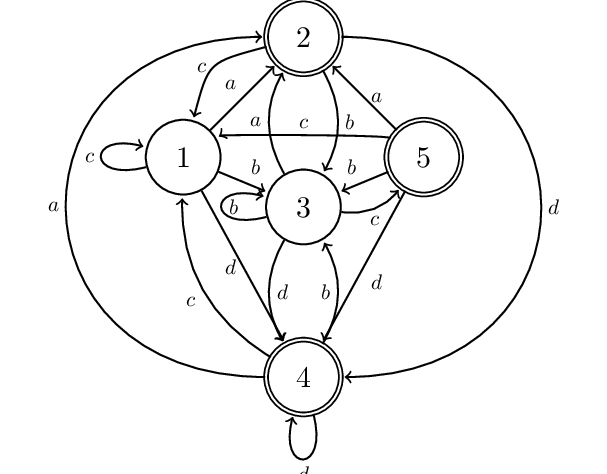
\includegraphics[width=0.5\textwidth]{images/dfa.png}
	\caption{A representation of a DFA.}
	\label{fig:DFA}
\end{figure}

A DFA can be exactly in one state at a given time and it makes the transition from one state to another state given some input and according to the transition function.


\section {Markov Decision Process} %DONE

Reinforcement learning is an area of machine learning which aims to learn an agent in order to maximize the total amount of reward, obtained form a complex, uncertain environment. 

The agent must have a model of the actions that can be taken into the environment in which it acts, in order to be able to explore/interact with the environment itself. But the agent, during learning phase, is not told which actions to take, instead it must discover which actions yield the most reward by trying them. Moreover, actions taken might affect not only immediate reward, but also subsequent ones leading to delayed rewards. The agent in this way can learn its behaviour inside the specific environment incrementally, using its own experience of errors and successes.
This is trial-and-error approach is widely discussed by Sutton and Barto in \textit{Reinforcement Learning: An Introduction} \cite{sutton2018rl}.
\\
Typically the way in which the agent interact with the environment is modeled as shown in figure \ref{fig:RL} also known as the Markovian stochastic control process, or Markov Decision Process (MDP).
\begin{figure}[h]
	\centering
	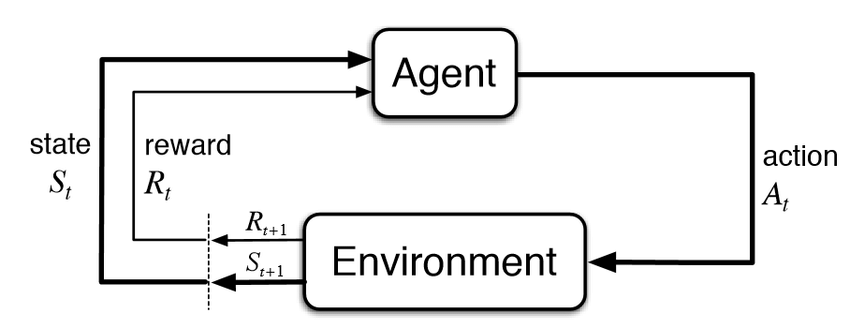
\includegraphics[width=0.6\textwidth]{images/rl_sutton_barto.png}
	\caption{Reinforcement Learning: agent-environment interaction.}
	\label{fig:RL}
\end{figure}

Markov Decision Processes provide a mathematical model for decision making in a non-deterministic environment. A MDP can be defined as the tuple $\langle S, A, T, R, \gamma \rangle$, where $S$ is the set of states $A$ is the set of actions, $T$ is a transition model, $R$ is a reward function and $\gamma$ as discount factor of the reward. 
\\
The transition model $T : S \times A \rightarrow P(S)$ is a function that given a tuple of state and action returns a distribution over the next state $s'$:
\begin{equation}
    T(s,a) = P(s',r,t|s,a)
\end{equation}
where $t$ is the terminal state, pointing that the agent reached a certain goal.
\\
The reward function $R : S \times A \rightarrow \R$, given an action $a$ in state $s$ returns a real valued reward of the action performed by the agent.

In MDPs the agent at time $t$ interacts with the environment choosing an action $a_t\in A(s)$, obtaining a reward $r_{t+1}$ and reaching a state $s_{t+1}$. These interactions are performed in discrete timesteps $t = 0,1,2,\dots$ generating a \textit{trajectory} $s_0, a_0, r_1, s_1, a_1, \dots$ shown in figure (\ref{fig:markov_assumption}).
\begin{figure}[H]
	\centering
	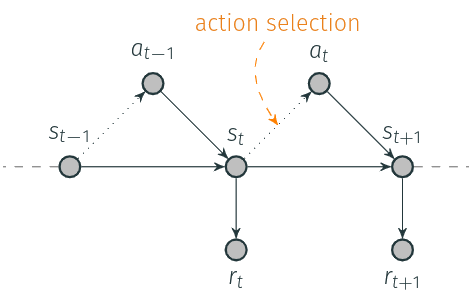
\includegraphics[width=.7\textwidth]{images/markov_assumption.png}
	\caption{Markov trajectory.}
	\label{fig:markov_assumption}
\end{figure}

In this model, given the present state $s_t$ all the following states are independent of all past states, meaning that there are no dependencies between a state $s_t+1$ and $s_{t-i}$ with $i=1,\dots,k$ as shown in figure (\ref{fig:markov_assumption}). This property is known as the \textbf{Markov assumption}, which states:
\begin{equation}
    s_{t+1}  \perp  s_0, \dots , s_{t-1} | s_t \quad \forall t
\end{equation}
\begin{equation}
    r_{t+1} \perp  s_0, \dots , s_{t-1}| s_t \quad \forall t
\end{equation}

After describing the mathematical model, the next step is to choose a method for action selection. The way in which the agent selects actions, given a state, is due to a function called policy $\pi : S \rightarrow A$. Learning a policy that allows the agent to maximize the total amount of reward received is the goal of Reinforcement Learning. 

To find an optimal policy $\pi ^*$, we have to maximize an expected return, which consider all the reward, not only obtained with the current action, but also the ones that we expect to obtain in the future. This is the value function $V:S \rightarrow \R$:
\begin{equation}
    V^\pi(s) = \EX \bigg[\sum_{k=0}^{\infty} \gamma^k r_{t+k} | s,\pi\bigg]
\end{equation}

Therefore, the optimal expected return can be defined as:
\begin{equation}
    V^*(s) = \max V^\pi (s)
\end{equation}

\noindent
Although state-values suffice to define optimality, it is useful to define action-values $Q$ function $Q:S \times A \rightarrow \R$, which computes the expected return starting in $s$, taking an action $a$ and then following the policy $\pi$:
\begin{equation}
    Q^\pi(s,a) = \EX \bigg[ \sum_{k=0}^{\infty} \gamma^k r_{t+k} | s,a,\pi  \bigg]
\end{equation}

As for the value function, the optimal $Q-value$ function is defined as:
\begin{equation}
    Q^*(s,a)= \max Q^\pi(s,a)
\end{equation}

In summary, the knowledge of the optimal action-value function alone suffices to know how to act optimally.


\section{Q-learning}\label{sec:ql} %DONE
Q-learning, proposed by Watkins and Dayan  \cite{watkins1992qlearn} in 1992 is a model-free reinforcement learning algorithm to learn the value of an action in a particular state. It does not require a model of the environment, and it can handle problems with stochastic transitions and rewards without requiring adaptations.

For any finite Markov Decision Process (FMDP), Q-learning finds an optimal policy $\pi$ in the sense of maximizing the expected value of the total reward over any and all successive steps, starting from the current state, $Q^\pi(s,a)$. Q-learning can identify an optimal action-selection policy for any given FMDP, given infinite exploration time and a partly-random policy. 
The optimal Q-function $Q^*(s,a)$ is the maximum return that can be obtained starting from observation $s$, taking action $a$ and following the optimal policy thereafter. 

The algorithm, therefore, has a function that calculates the quality of a state–action combination:
\begin{equation}
    Q:S\times A \rightarrow \mathbb{R}
\end{equation}
$Q$ is in general randomly initialized. During the execution of the algorithm the agent at time $t$, in a state $s_t$, selects an action $a_t$\footnote{Q-learning is an off-policy algorithm that learns about the \textit{greedy policy} $a_t = \max_{a_{t+1}} Q(s_{t+1},a_{t+1})$ while using a different \textit{behaviour policy} for acting in the environment/collecting data. This \textit{behaviour policy} is usually an $\varepsilon$-greedy policy that selects the greedy action with probability $(1-\varepsilon)$ and a random action with probability $\varepsilon$ to ensure good coverage of the state-action space.} and observes a reward $r_t$ entering in a new state $s_{t+1}$. 

 
The optimal Q-function obeys the Bellman optimality equation:
\begin{equation}
    Q^*(s_t,a_t) = \mathbb{E}\big[r_t+\gamma \max_{a_{t+1}} Q^*(s_{t+1},a_{t+1})\big]
\end{equation}

The basic idea behind Q-Learning is to use the Bellman optimality equation as an iterative update to maximize the expected value:
\begin{equation}
    Q(s_t,a_t)'\leftarrow (1-\alpha)Q(s_t,a_t)+\alpha (r_t+\gamma \max_{a_{t+1}} Q(s_{t+1},a_{t+1}))
\end{equation}
where $\alpha$ is the learning rate and $\gamma$ is the discount factor. The new Q-table values $Q(s_t,a_t)'$ are given by the terms:
\begin{description}
\item[$(1-\alpha)Q(s_t,a_t)$]: the current value weighted by the learning rate. Values of the learning rate near to 1 make the changes in 
Q more rapid.
\item[$\alpha\max_{a_{t+1}} Q(s_{t+1},a_{t+1})$]: the maximum reward that can be obtained from state 
$s_{t+1}$, weighted by learning rate and discount factor.
\item[$\alpha r_t$]: the reward weighted by the learning rate.
\end{description}
The discount factor has the effect of valuing rewards received earlier higher than those received later.

\begin{figure}[ht]
    \centering
    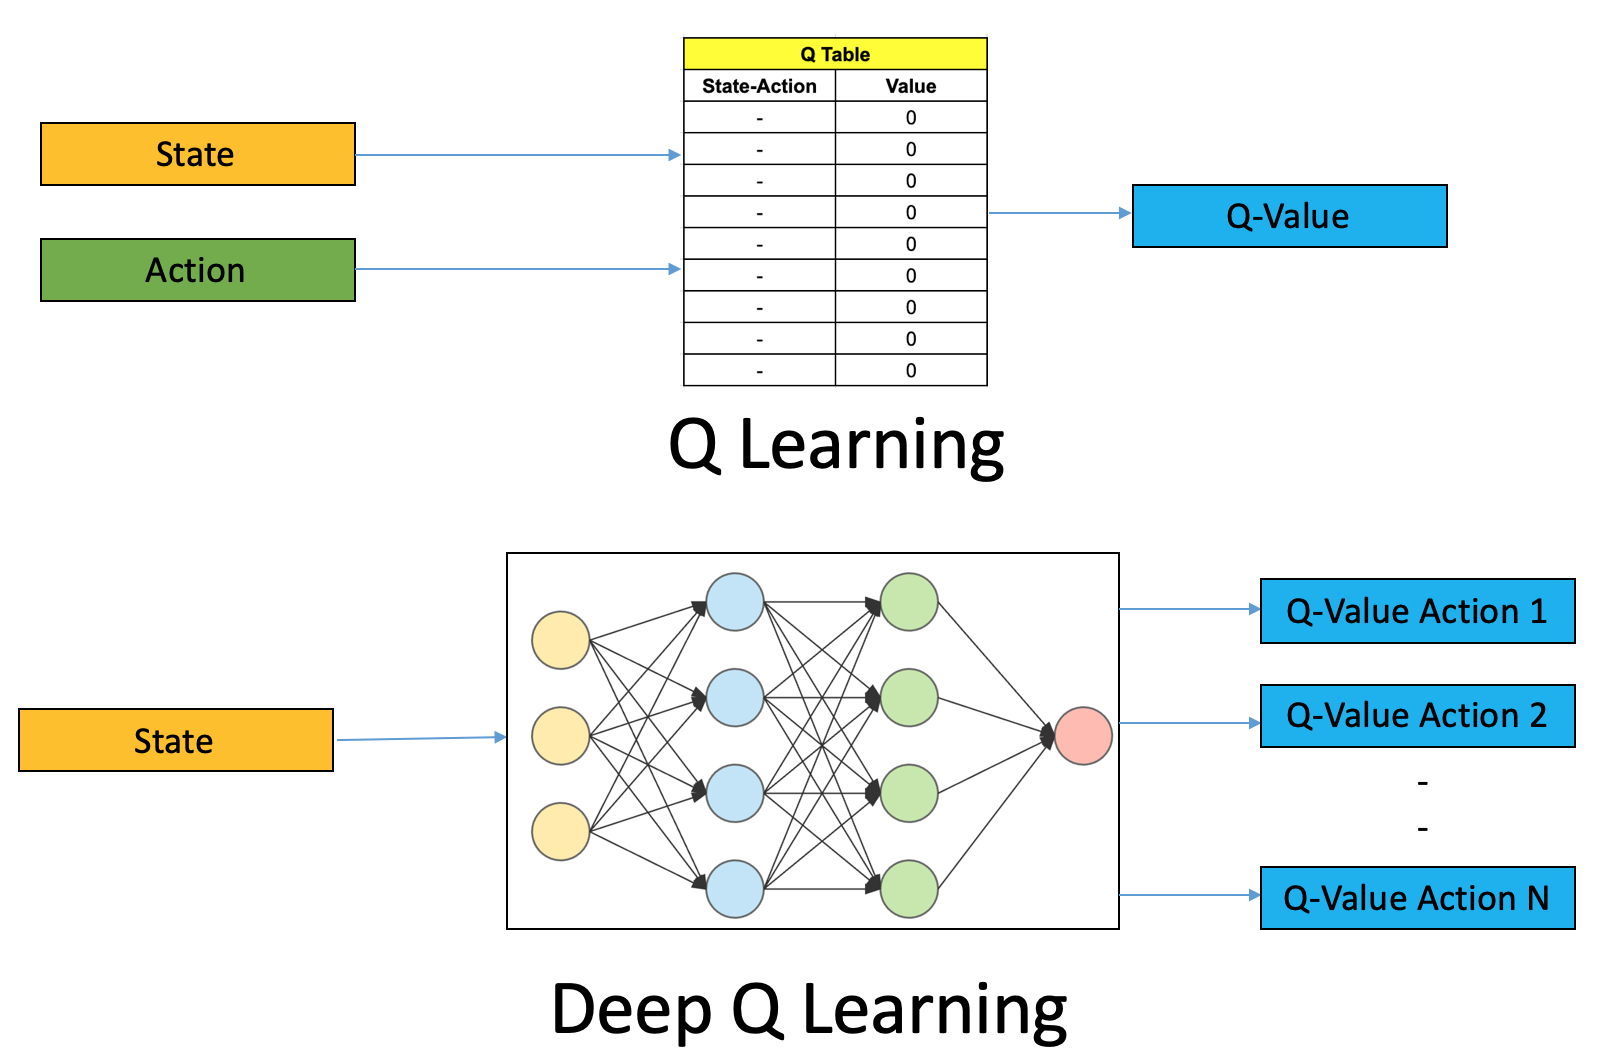
\includegraphics[width=0.7\textwidth]{images/q-dqn.png}
    \caption{The conceptual difference of Q-learning and Deep Q-learning. Form the Q-table we get the Q-value from a (state,action) pair. In a DQN the neural network produces a Q-value distribution over the actions, its maximum value correspond to the best action to take.}
    \label{fig:qdqn}
\end{figure}
\subsection{Deep Q-Network}\label{sec:dqn} %DONE

The DQN (Deep Q-Network) algorithm was developed by DeepMind \cite{Mnih2015HumanlevelCT} in 2015. It was able to solve a wide range of Atari games (some to superhuman level) by combining reinforcement learning and deep neural networks at scale. The algorithm was developed by enhancing a classic RL algorithm called Q-learning with deep neural networks and a technique called \textit{experience replay}. "Q" refers to the function that the algorithm computes, the expected rewards for an action taken in a given state.

The core difference between Deep Q-learning and Vanilla Q-learning is the \textit{agent brain}, Figure \ref{fig:qdqn}. Critically, Deep Q-learning replaces the regular Q-table with a neural network. Rather than mapping a state-action pair to a \textit{q-value}, a neural network maps input \textit{states} to (\textit{action}, \textit{q-value}) pairs in order to estimate the optimal Q-table. Such approach is particularly suited when dealing with problems in which it is impractical to represent the Q-function as a table containing values for each combination of states and actions, i.e. continuous space domains. 

The DQN learns a function approximator (a neural network with parameters $\theta$), to estimate the Q-values, i.e. 
$Q(s,a;\theta)\approx Q^*(s,a)$, by minimizing the temporal distance error using the loss at each step $i$:
\begin{equation}
    L_i(\theta_i)=\mathbb{E}\big[(r_t+\max_{a_{t+1}} Q(s_{t+1},a_{t+1};\theta_{i-1})-Q(s_{t},a_{t};\theta_{i}))^2\big]
\end{equation}
which is minimized for $Q(s_{t},a_{t};\theta_{i})\approx r_t+\max_{a_{t+1}} Q(s_{t+1},a_{t+1};\theta_{i-1})$ meaning that the estimated Q-values are as close as possible to the expected reward discount (this and the next reward), i.e. if this condition holds for every state (the loss is minimized) then we have the optimal Q-table. Minimization is performed by using stochastic gradient descent over mini-batches of \textit{experience replay}.

\subsubsection{Experience Replay}\label{sec:exrep}%DONE

The DQN work by DeepMind introduced a technique called Experience Replay to make the network updates more stable. At each time step of data collection, the transitions are added to a circular buffer called the \textit{replay buffer}. Then during training, instead of using just the latest transition to compute the loss and its gradient, they are computer by using a mini-batch of transitions sampled from the \textit{replay buffer}. This has two advantages: better data efficiency by reusing each transition in many updates, and better stability using uncorrelated transitions in a batch.



% The DeepMind system used a deep convolutional neural network, with layers of tiled convolutional filters to mimic the effects of receptive fields. Reinforcement learning is unstable or divergent when a nonlinear function approximator such as a neural network is used to represent Q. This instability comes from the correlations present in the sequence of observations, the fact that small updates to Q may significantly change the policy of the agent and the data distribution, and the correlations between Q and the target values.

% The technique used experience replay, a biologically inspired mechanism that uses a random sample of prior actions instead of the most recent action to proceed.[2] This removes correlations in the observation sequence and smooths changes in the data distribution. Iterative updates adjust Q towards target values that are only periodically updated, further reducing correlations with the target.[17]

\section{Non Markovian Rewards Decision Processes}%DONE
A Non Markovian Decision Process (NMDP) is, as the name suggests, a stochastic process that does not exhibit the Markov properties (\cite{Thiebaux06}). The reward in this case is different in that it depends on the history of visited states, and its domain is a set of finite state sequences drawn from S, denoted as $S^*$. 

A general function for a Non Markovian Reward can be stated as going from $(S \times A)^* \rightarrow \mathbb{R}$ [\cite{camacho_chen_sanner_mcilraith_2017}]. Similar to the reward function, the policy for an NMRDP depends on history, and can be identified as a mapping from $S^*$ to $A$. An NMRDP can be represented as a Tuple $\langle S, A, Tr, R \rangle$ where $S$, $A$, $Tr$ as the same as in an MDP, and $R$ is reinterpreted as described in the previous paragraph.  

A main problem that occurs with NMRDP is that the reward may not be stationary and thus it (along with the optimal policy $\rho^*$) cannot be computed normally. To solve this we can define an MDP that is equivalent to the Non Markovian one (this can be seen in "The non markovian agent" section \ref{sec:non_mark_agent} later on). \\

\subsection{LTLf/LDLf}%DONE
To better express temporal properties over sequences of states we can use Linear Temporal Logic ($LTL$) [\cite{brafman2018ltlf_LTLF_LDLF}] which is a language that allows us to encode automaton information into formulae $\varphi$ that balance expressiveness with ease of use. We can use $LTL_f$ (a variant of $LTL$ expressed over finite states) to describe Markovian rewards, as well as construct a corresponding $DFA$ ($A_\varphi$) that accepts a sequence of states $\pi$ if and only if it satisfies $\varphi$ (\cite{camacho_chen_sanner_mcilraith_2017}).

In the case of non-Markovian rewards, we need to introduce a new formalism: $LDL_f$, \textit{Linear Dynamic Logic over finite traces}. $LDL_f$ is an extension of $LTL_f$, including Regular Expressions in the temporal formulas, as we can see in the equations \ref{eq:ltlf_ldlf}.

\begin{align}
    \varphi &::= tt|ff|\neg \varphi | \varphi_1 \wedge \varphi_2| \langle \varrho \rangle\varphi | [\varrho]\varphi \nonumber\\ 
    \varrho &::= \phi | \varphi? | \varrho_1 + \varrho_2 | \varrho_1 ; \varrho_2 | \varrho^* 
    \label{eq:ltlf_ldlf}
\end{align}
where $tt$ and $ff$ stand for \verb|true| and \verb|false|; $\phi$ is a propositional formula on current state; $\neg \varphi, \varphi_1 \wedge \varphi_2$ are boolean connectives; $\varrho$ is a regular expression on propositional formulas $\phi$ with the addition of the test construct $\varphi?$; $\langle \varrho \rangle\varphi$ says that exists an execution of the Regular Expression (RE) $\varrho$ that ends with $\varphi$ holding; $[\varrho]\varphi$ states that all executions of RE $\varrho$ along the trace end with $\varphi$ holding.

It is more expressive than the Linear Time Logic, as it caputres Monadic Second-Order Logic ($MSO$) instead of First-Order Logic ($FOL$).

%%%%%%%%%%
% \section{Non Markovian Rewards Decision Processes}
% A Non Markovian  Decision Process is a stochastic process that does not exhibit the Markov properties [\ref{one}],
% [\ref{two}] (generalized as  memoryless property).
% A Non Markovian Reward Decision Process (NMRDPs) is a tuple $M= \langle S, A, T, R, \gamma \rangle$, where S,A, T, $\gamma$ are equivalent to MDPs case, while R is redefined as $\bar{R}:(S\times A)^* \longrightarrow \mathbb{R}$.\\
% Now  the reward  is a real valued function over finite state-action sequences (according to a specific history).

% \paragraph{Temporal rewards specifications}
% \noindent\\\\
% In these cases, we have a set of episodes (traces $\pi$), in fact the temporal logics needs to talk about set of temporal traces.
% The concept is the following: we have a temporal formula $\phi$ and we can observe all traces that satisfy this formula.
% The steps are the following:
% \begin{itemize}
% \item Define an alphabet of propositional symbols (fluents)
% \item Define labelling function $f_F:S\times A \longrightarrow 2^F$
% \end{itemize}
% \noindent
% These definitions induce a trace $\pi$ of propositional interpretations:\\ $ (S\times A)^*\xrightarrow{f_F}  (2^F)^*$.\\
% In order to define the non-markovian reward, we firstly define a set of formulas with associated reward $\{(\phi_i,r_i)\}_{i=1} ^m$.
% Then  the non-markovian reward is :\\

% \begin{figure}[h]
%   \centering
% \includegraphics[scale=0.65]{images/NMreward.png}\\
% \end{figure}

% \noindent
% in particular, if episode (trace $\pi$) satisfies formula $\phi$ it generates a reward.

% \paragraph{Rewarding with automata}\\
% \noindent\\\\
% Any LTLf/LDLf formula $\phi$ can be converted to DFA that recognizes the same traces ($A_\phi=\langle Q_\phi, q_{o\phi},\Sigma, F_\phi\rangle$). Practically we can translate Non-Markovian Rewards Decision Process into a MDP with state space:
% $S'= S \times Q_{\phi(1)}\times .... \times Q_{\phi(m)}$\\
% \noindent
% This is a cross product, where $S$ is the set of states and $Q_{\phi(i)}$ (with $i=1,..,m$) are the automaton states.

\section{Counterfactual Experiences for Reward Machines (CRM)}\label{sec:CRM}%DONE

\begin{figure}[ht]
    \centering
    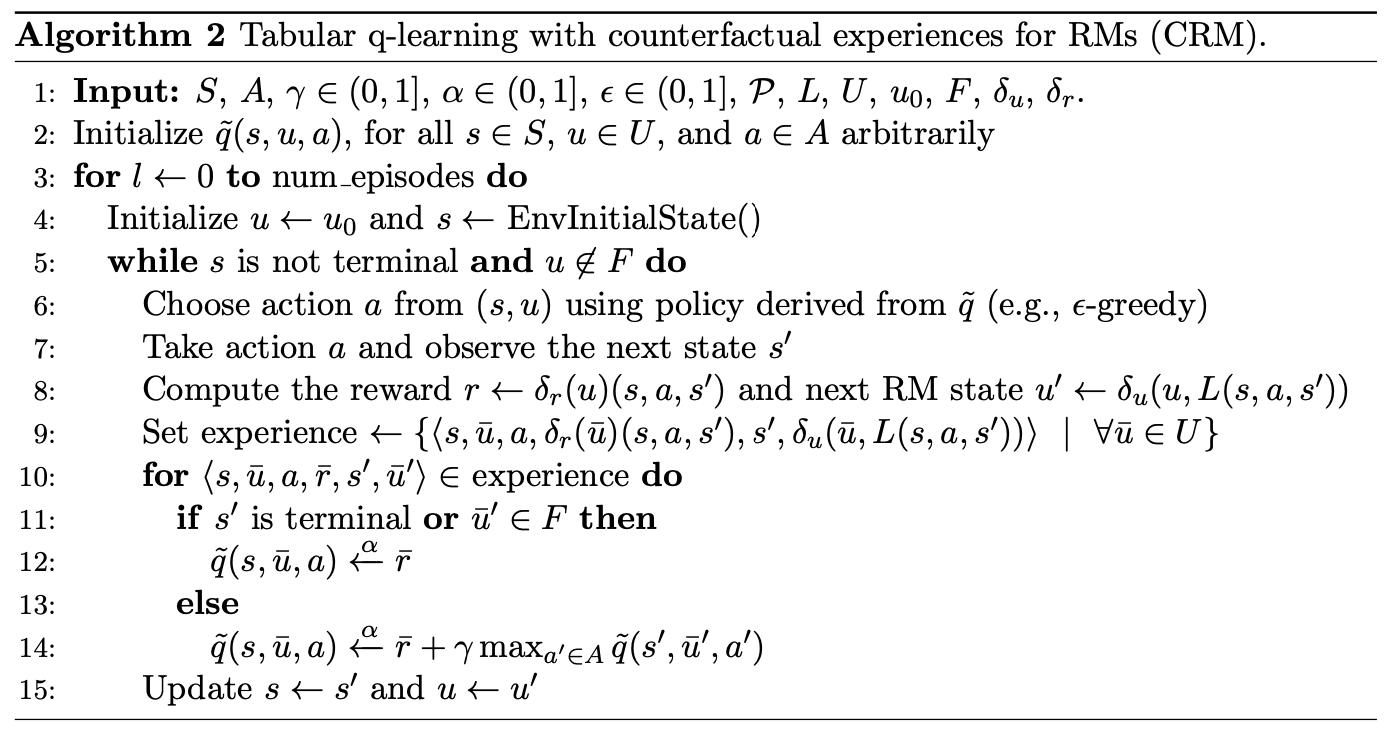
\includegraphics[width=0.95\textwidth]{images/CRM_alg2.png}
    \caption{Adaptation example of CRM method to tabular q-learning (off-policy learning) with the addition of lines 9 and 10.}
    \label{fig:crm_alg}
\end{figure}

\textit{Counterfactual Experiences for Reward Machines (CRM)} is an algorithm from \cite{icarte2020reward} which exploit the information in the reward machine (RM) to facilitate learning. It aims at learning policies $\pi(a|s,u)$ (with $\pi$ the agent's policy, $a$ the distribution over the actions, $s$ the observation and $u$ the reward machine state) but uses counterfactual reasoning to generate \textit{synthetic experiences}.

This algorithm is easily extendable to work with deep RL agents. In fact these experiences can then be used by an off-policy learning method, such as tabular Q-learning, DQN, or DDPG, to learn the policy $\pi(a|s,u)$ faster.

The key idea behind CRM is about enhancing the exploration of the reward machine state space, it allows the agent to reuse experience to learn the right behaviour at different RM states. Given the cross-state $\langle s,u\rangle$, the agent perform an action $a$ and observe the new cross-state $\langle s',u'\rangle$ and get a reward $r$. We can exploit the reward machine to experience more outcomes of the cross-state and speed up the training. In fact after have performed the actual experience $\langle s,u,a,r,s',u'\rangle$, we can accumulate more experience collecting, for each RM state $\bar{u}\in U$, the resulting rewards $\bar{r}$ and outcomes $\bar{u}$ and generate the set of experiences:
\begin{equation} \label{eq:crm}
   \big\{ \langle s,\bar{u},a,\bar{r},s',\bar{u}'\rangle\; | \;\forall \bar{u}\in U \big\}.
\end{equation}
An example of possible implementation for tabular Q-learning is shown in Figure \ref{fig:crm_alg}. For both DQN and DDPG, the counterfactual experiences would simply be added to the experience replay buffer and then used for learning as is typically done with these algorithms.

To better understand the content we can look at the example in Figure \ref{fig:examp_crm} 

\begin{figure}[h]
    \centering
    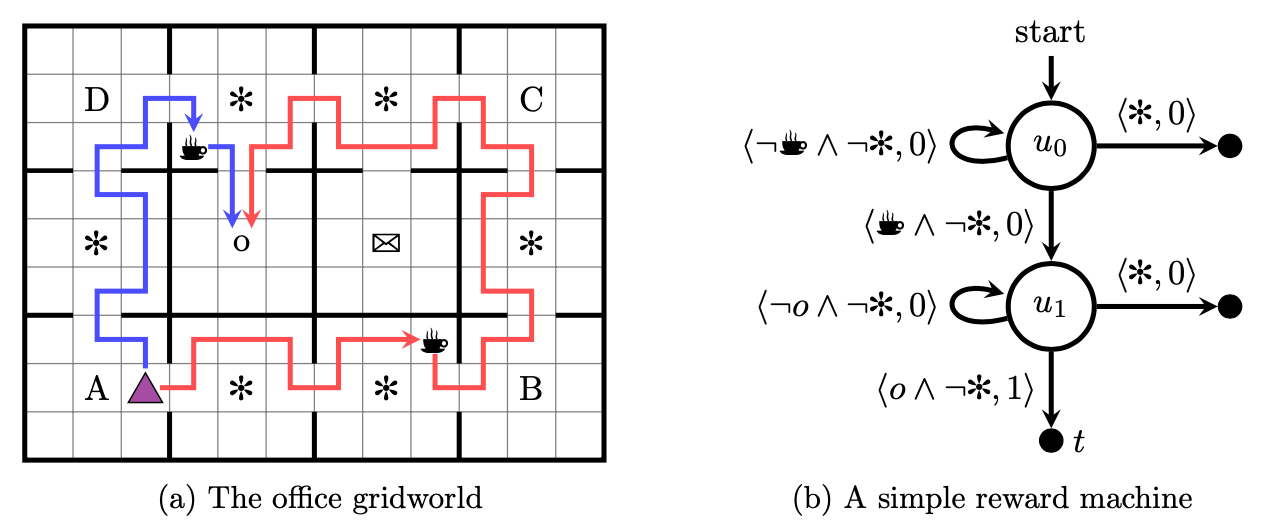
\includegraphics[width=0.95\textwidth]{images/examp_CRM.png}
    \caption{An example environment (a) and one reward machine for it (b) i.e. get coffee, then reach office.}
    \label{fig:examp_crm}
\end{figure}

Suppose that the agent gets to the office before getting the coffee. The Q-learning baseline would use that experience to learn that going to the office is not an effective way to get coffee. In contrast, Q-learning with CRM would also use that experience to learn how to get to the office. As such, CRM will already have made progress towards learning a policy that will finish the task as soon as it finds the coffee, since it will already have experience about how to get to the office.

CRM also converges to optimal policies when combined with q-learning and this is a theorem in \cite{icarte2020reward}:

\textbf{Theorem}. Given an MDPRM (Markov Decision Process with Reward Machine), CRM with tabular q-learning converges to an optimal policy for the problem in the limit (as long as every state-action pair is visited infinitely often).

While the convergence proof for CRM is directly given as a consequence of the convergence proof provided by \cite{watkins1992qlearn} for tabular q-learning when we consider that the experience is sampled according to the its transition probability $p(\langle s', u'\rangle|\langle s, u\rangle, a) = p(s'|s, a)$.

\section{Gym-Sapientino} %DONE
This is a new RL discrete environment that respects the gym interface\footnote{https://github.com/cipollone/gym-sapientino-case}.
\noindent
In this environment, we have a planar unicycle robot that can move inside a 2-D grid, which is basically a rectangular map with some coloured cells, as depicted in Figure \ref{fig:sapientino_grid}. The goal of the agent-robot is to visit the coloured cells of a continuous state space in a specific order. SapientinoCase has a low–dimensional observation space, which allows to use simple Feed–Forward Neural Networks.

\begin{figure}[h]
    \centering
    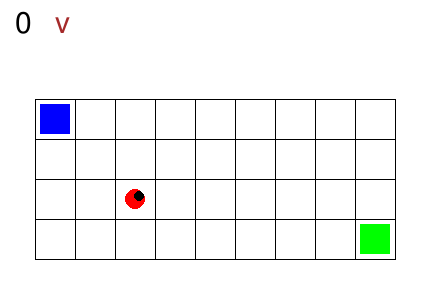
\includegraphics[width=0.7\textwidth]{images/sapientino.png}
    \caption{Gym-Sapientino environment.}
    \label{fig:sapientino_grid}
\end{figure}

Moreover also the observations received from the environment are continuous. The observations that are continuous on the state, are characterized by the \textit{position}, the \textit{linear velocity} and  the \textit{angular velocity}. \\
After an action executed by the agent executes an action, the environment returns an associated reward and an observation on the state and on automaton state.


\subsection{Temporal Goal on Gym-Sapientino} %TOBEREVIEWED

The non markovian agent moves in the map executing a non markovian task: visit a sequence of cells identified by colors, in a specified order. % (the ordered visit of a sequence of colors)
Essentially the agent should be prone to reach some temporal goals, identified by the sequence of colors like.
\\
When the agent reach a temporal goal it receives a specific reward from the environment, moreover following the temporal goals it will accumulate an amount of rewards. Therefore more frequently the agent earns rewards more it will be led to learn.
\\
This environment allows to work with four different colors ( and consequently with a temporal goal characterized by four components): \textbf{yellow}, \textbf{blue}, \textbf{green} and \textbf{red}.
\\
An example of temporal reward inside the \textit{Gym-Sapientino} environment is $LDL_f$ formula:
\texttt{<!red*; red; !green*; green; !blue*; blue>end}.

\noindent
%Gym-Sapientino uses LYDIA in order to convert temporal goals into automata.
It is possible to specify which colors are included in the temporal goal formulas $\phi$, and consequently in the related automaton $A_\phi$ (which is provided by the environment). 
In the automaton the states related to the colors are specified through numbered codification. In the previous version of \textit{Gym-Sapientino} there was a particular failure state, denoted as \verb|SINK|. In the new version of this environment this variable is removed and therefore the dfa is sequential, therefore if we consider a map characterized by two colors, for instance \textit{blue} and \textit{green}, the related automaton will no longer have a frozen set as shown by figures (\ref{fig:sinkdfa}) and (\ref{fig:nosinkdfa}).\\

\vspace{2em}
\begin{figure}[H]
\begin{minipage}{.5\textwidth}
  \centering
  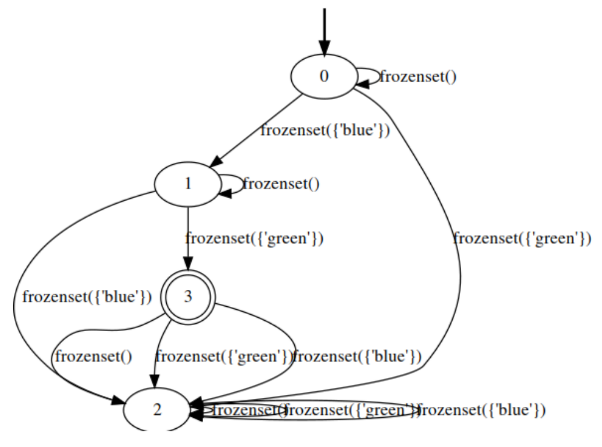
\includegraphics[width=1\linewidth]{images/old_dfa2colors.png}
  \caption{Old DFA with sink state.}
  \label{fig:sinkdfa}
\end{minipage}%
\begin{minipage}{.5\textwidth}
  \centering
  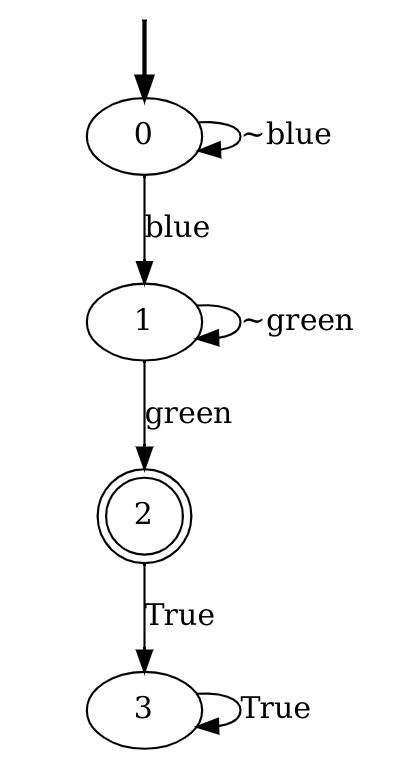
\includegraphics[width=.38\linewidth]{images/dfa2colors.png}
  \caption{New DFA without sink state.}
  \label{fig:nosinkdfa}
\end{minipage}
\end{figure}


\noindent
Notice that \texttt{0} is the initial state and \texttt{2} is the accepting state.
In this case the agent can reach the temporal goal visiting the following sequence: \texttt{0,1,2}. 

% In order to control the correct achievement of the temporal goal, we have also interfaced with the following problem:\\
% in Gym-Sapientino environment the agent can execute some actions signaled by five particular  strings: \texttt{LEFT}, \texttt{RIGHT}, \texttt{FORWARD}, \texttt{NULL}, \texttt{BEEP}. The first,the second and the third need to indicate in which direction the agent is moving, the fourth needs to signal that the agent is not moving and the last needs to signal that the agent is visiting a certain state.
% The problem rises when the agent enters in the same state twice consecutively, and this implies a double \texttt{BEEP} visualization. In our work we have controlled this problem, avoiding that the current state reached by the agent was equal to the previous reached state. In this case we impose that the temporal goal is satisfied only when the sequence of states does not include equal states. For instance in the previous example with two colors ( blue and green):\\
% the temporal goal is reached when this sequence is visited \texttt{0,1,3} and not \texttt{0,1,1,3} or \texttt{0,1,3,3}.




%\section{Reward shaping}
%Most of the techniques in Reinforcement Learning (RL) assumes that the learning starts from a blank slate and improves only by means of trial and error. This learning approach takes a huge amount of trials and as a direct consequence it implies that the time required is a lot. This is why we talk about \textbf{reward shaping} \citep{rf}. This method is useful to incorporate domain knowledge in the RL agents. In reward shaping, the domain knowledge is represented as a supplementary reward that allows the RL agent to learn more efficiently.
%A Deterministic Finite Automaton (DFA) \citep{dfa} is a mathematical model that maps an input sequence to an output. The result is that the computation is unique. A DFA can be exactly in one state at a given time and it makes the transition from one state to another state given some input and according to the transition function.\\
%In our code the \textbf{Reward shaping} has been implemented and applied as showed in \ref{fig:reward shaping}, where according to \ref{fig:stati} the agent received a great reward of 500 when reaching the right state, otherwise in case of \textit{SINK\_ID} the reward is -500.

%\vspace{2em}
%\begin{figure}[H]
%\centering
%\includegraphics[width=\linewidth]{rs}
%\caption{Reward shaping}
%\label{fig:reward shaping}
%\end{figure}

\section{The non markovian agent}\label{sec:non_mark_agent} %DONE
Our main focus is to have an agent go through a specific state sequence such that it passes through the blue square first, then the red square, and finally end on the green square. Thus meaning that to get to the goal state in sequence we have to have passed through all the previous ones in order. This sequence of events therefore requires the agent to know where it has been in the past, making it a non markovian problem, and, in turn, a non markovian agent. 
However, as stated in the NMDRP section before, it is much easier to compute a system that behaves in a Markovian way. \\

\begin{figure}
    \centering
    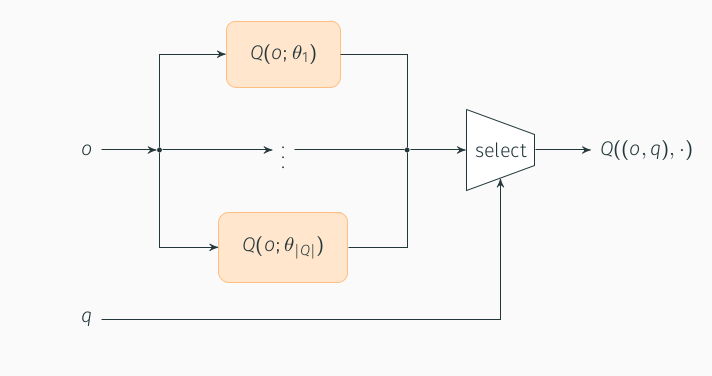
\includegraphics[width=0.7\textwidth]{images/baseline_implementation_schema.png}
    \caption{Baseline implementation of a non markovian policy network. It takes as input the observation \(o\) and the state of the goal DFA \(q\). Then, according to the state of the automaton, the agents selects one of the \(|Q|\) \textit{separate experts} for the action selection. This image is taken from the slides of PhD student Roberto Cipollone for the Reasoning Agent course held in Sapienza in 2020/2021.}
    \label{fig:baselineSchema}
\end{figure}



\noindent
To allow us to create a Markovian problem from our task we split it into smaller parts. Hence the new problem becomes a combination of smaller sub-tasks, instead of having the agent follow the full sequence, we will have it reach the individual states. The first sub-task will require the agent to reach the blue square, the second the red, and the third the green. By doing this we remove the dependency on history, as each problem is treated individually, and we create three separate Markovian problems out of a non Markovian one. \\

%---------------------------------------------

%However, at any given time, only one markovian agent can select an action to execute (figure [\ref{fig:baselineSchema}]). \\
%The action selection is constrained by the goal formulation. In fact, we consider the gym Sapientino task to be solved if and only if the non markovian agent visits the colors \textbf{in the order in which they appear in the temporal goal formula}. In fact, if the agent visits the colors in the wrong order (for example \{\textit{blue},\textit{green}, \textit{red}\} instead of \{\textit{blue}, \textit{red}, \textit{green}\}) 

%Sinks (?)
%the automaton goes in the \textit{sink} state and episode terminates with a failure.\\

\noindent
%To reach the goal,then, the agent must be aware of which color in the goal sequence it has already visited and which color is the next one in the sequence. Such an information may be inferred by inspecting the states of the goal DFA. (see the example in figure [\ref{fig:stati}].
%(riferimento alle figure dei goal DFA)
%In fact, once the agent correctly visits a portion of the formula (\color{blue} blue \color{black} for the problem considered), the DFA changes the state. If the resulting state is accepting, it means that the agent has visited the whole formula; otherwise there are still some colors to visit.\\%
%Luckily the environment allows the agent to keep track of the automaton states. 
%Therefore, in order to visit the goal, it is sufficient to select, from time to time, the "correct" markovian agent depending on the automaton state (see figure [\ref{fig:nonMarkovianNetwork}] for a  graphical explanation) .
\noindent




%The code below is based on the tutorial https://latexdraw.com/drawing-neural-networks-in-tikz-short-guide/

%Define the number of input neurons.
\newcommand{\inputnum}{7}

%Define the number of hidden neurons.
\newcommand{\hiddennum}{9}

%Define the number of output neurons.
\newcommand{\outputnum}{5}


%Define the position on the x-axis of the first hidden layer neurons.
\newcommand{\firstHiddenNeuronsPosition}{3.0}


%Define the position on the x-axis of the second hidden layer neurons.
\newcommand{\secondHiddenNeuronsPosition}{6.0}


%Define the position on the x-axis of the output layer neurons.
\newcommand{\outputNeuronsPosition}{9.0}

%Define the position of the oneHotEncoding for the first hidden layer.
\newcommand{\oneHotEncodingFirstHidden}{3.5}


%Define the position of the oneHotEncoding for the second hidden layer.
\newcommand{\oneHotEncodingSecondHidden}{6.5}



%Define the number of output neurons.


\begin{figure}

\begin{tikzpicture}[x=1.5cm, y=1.5cm, >=stealth]


%Input neurons
\foreach \i in {1,...,\inputnum}
{
    \node[circle, 
		minimum size = 6mm,
		fill=orange!30] (Input-\i) at (0,-\i) {};
}

%First hidden layer.
\foreach \i in {1,2,3}
{
    \node[circle, 
		minimum size = 6mm,
		fill=blue!50,
		yshift =(\hiddennum-\inputnum)*5mm] (Hidden-\i) at (\firstHiddenNeuronsPosition,-\i) {};
}

\foreach \i in {4,5,6}
{
    \node[circle, 
		minimum size = 6mm,
		fill=red!50,
			yshift =(\hiddennum-\inputnum)*5mm] (Hidden-\i) at (\firstHiddenNeuronsPosition,-\i) {};
}

\foreach \i in {7,8,9}
{
    \node[circle, 
		minimum size = 6mm,
		fill=yellow!50,
			yshift =(\hiddennum-\inputnum)*5mm] (Hidden-\i) at (\firstHiddenNeuronsPosition,-\i) {};
}


%One hot encoding for the first hidden layer
\foreach \i in {1,2,3}
{
 \node[circle, 
		minimum size = 6mm,
		fill=gray!30,
			yshift =(\hiddennum-\inputnum)*5mm] (OneHotHidden1-\i) at (\oneHotEncodingFirstHidden,-\i) {1};

}


\foreach \i in {4,5,6,...,9}
{
 \node[circle, 
		minimum size = 6mm,
		fill=gray!30,
			yshift =(\hiddennum-\inputnum)*5mm] (OneHotHidden1-\i) at (\oneHotEncodingFirstHidden,-\i) {0};

}



%Second hidden layer.
\foreach \i in {1,2,3}
{
    \node[circle, 
		minimum size = 6mm,
		fill=blue!50,
			yshift =(\hiddennum-\inputnum)*5mm] (Hidden2-\i) at (\secondHiddenNeuronsPosition,-\i) {};
}

\foreach \i in {4,5,6}
{
    \node[circle, 
		minimum size = 6mm,
		fill=red!50,
			yshift =(\hiddennum-\inputnum)*5mm] (Hidden2-\i) at (\secondHiddenNeuronsPosition,-\i) {};
}

\foreach \i in {7,8,9}
{
    \node[circle, 
		minimum size = 6mm,
		fill=yellow!50,
			yshift =(\hiddennum-\inputnum)*5mm] (Hidden2-\i) at (\secondHiddenNeuronsPosition,-\i) {};
}



%One hot encoding for the second hidden layer
\foreach \i in {1,2,3}
{
    \node[circle, 
		minimum size = 6mm,
		fill=gray!30,
			yshift =(\hiddennum-\inputnum)*5mm] (OneHotHidden2-\i) at (\oneHotEncodingSecondHidden,-\i) {1};
}
\foreach \i in {4,5,6,...,9}
{
    \node[circle, 
		minimum size = 6mm,
		fill=gray!30,
			yshift =(\hiddennum-\inputnum)*5mm] (OneHotHidden2-\i) at (\oneHotEncodingSecondHidden,-\i) {0};
}

%Output layer.
\foreach \i in {1,...,\outputnum}
{
    \node[circle, 
		minimum size = 6mm,
		fill=orange!30,
		yshift = (\outputnum-\inputnum)*5mm
		] (Output-\i) at (\outputNeuronsPosition,-\i) {};
}


% Connect neurons In-Hidden
\foreach \i in {1,...,\inputnum}
{
	\foreach \j in {1,...,\hiddennum}
	{
		\draw[->, shorten >=1pt] (Input-\i) -- (Hidden-\j);	
	}
}

% Connect neurons Hidden-Hidden2
\foreach \i in {1,...,\hiddennum}
{
	\foreach \j in {1,...,\hiddennum}
	{
		\draw[->, shorten >=1pt] (OneHotHidden1-\i) -- (Hidden2-\j);
	}
}


% Connect neurons Hidden2-output
\foreach \i in {1,...,\hiddennum}
{
	\foreach \j in {1,...,\outputnum}
	{
		\draw[->, shorten >=1pt] (OneHotHidden2-\i) -- (Output-\j);
	}
}








\end{tikzpicture}
\caption{Conceptual representation of the non markovian policy network used, a 2 hidden layer Multi Layer Perceptron (MLP). Notice that the hidden layers activates depending on the one hot encoded \color{gray} automata state \color{black} in input, this makes each set of perceptrons specialized in solving one automata state. The architecture in the figure may employed in solving the problem of visiting a sequence of three colors amid \color{blue} blue \color{black}, \color{red} red \color{black} and \color{yellow} yellow\color{black}. Color repetition is also applicable, the more the number of automata states the larger the hidden layers.}
\label{fig:nonMarkovianNetwork}
\end{figure}

\section{Implementation Details}\label{sec:ImplementationDetails}%DONE

The agent and its policy are implemented in Tensorforce\footnote{\url{https://tensorforce.readthedocs.io/en/latest/}}, an open source library for deep reinforcement learning based on Tensorflow and Keras. Tensorforce supports a variety of deep RL agents on-policy and off-policy like DQN, PPO, DDPG, etc. \\
Tensorforce is one of the most frequently used frameworks for reinforcement learning experiments. However, as far as we know, the latest version of the library (Tensorforce 0.6.5) does not support non markovian agents implementation by default. Therefore, for the purpose of our project, we must manipulate the Tensorforce agent policy networks and adapt them to a non markovian framework. In fact it permits to internally develop custom networks; it offers the implementation of most common neural network layers (dense, recurrent, convolutional, attention based) for policy network implementation.

\subsection{Network} %DOING
In this work, we propose a non markovian agent implementation inspired from the work in Figure \ref{fig:baselineSchema} about the \textit{separate experts} and from\footnote{\url{https://github.com/francycar/RA_project/tree/main}} which employs a single policy network for action selection divided in sets of neurons each defining a single markovian agent, see Figure \ref{fig:nonMarkovianNetwork}.
We make each chunk of the same size and associate it to a different color in the goal sequence. 

The network itself is very simple, a 2 hidden layers Multi Layer Perceptron (MLP). We have two inputs, the first is a 7-dimensional real input space (state space), while the second is a $num\_automata\times hidden\_size$-dimensional binary input, and a 5-dimensional real output space (action space). The binary input is created by one hot encoding of the automata state (using \textit{ones} for the current automata state correspondent neurons and \textit{zeros} otherwise), this is needed to gather the hidden neurons. In this way we are able to select the neurons, thus the current expert, which will contribute to the action selection.



% %Fare disegnino del vettore che si costruisce (?)

% \begin{enumerate}
%     \item Instantiate a vector filled with zeros of size \(H * N\) where \(N\) is the number of automaton states and \(H\) is the size of each \textit{chunk} of the policy network.
%     \item Divide the encoded state vector into equally sized sub-portions. Each portion will have a size of \(H\). The encoded state vector portions and the non markovian policy network \textit{chunks} described in the previous point must have the same size.
%     \item Assign the sub-portions to a different automaton state.
%     \item Fill the part corresponding to the \textbf{current automaton state} with \textit{ones} and leave the rest with \textit{zeros}.
%     \item Multiply the binary vector to the output of each dense layer to \textbf{select}, from time to time, the \textit{chunk} of the network of interest (a subset of the neurons of the dense layer).
%     \
% \end{enumerate}
% In this way we are able to select the chunks of the non markovian policy network which contribute to the action selection. In fact, the hidden layer neurons which are multiplied to 1 elements in the binary vector are kept in the forward pass and determines the action the policy network selects in the current state.\\ 
% On the other hand, the neurons of the network multiplied by the zeros in the binary vector do not contribute to the action selection (they are \textit{"zeroed"} ) and simply \textbf{get discarded}.\\
% Using this strategy, we are able to select all the network sub portions which correspond to the expert we would like to consider at any given time, discarding all the network chunks that correspond to the other experts (figure [\ref{fig:nonMarkovianNetwork}]).\\
% In figure [\ref{fig:nonMarkovianNetwork}] we show a graphical example of a forward pass in the non markovian policy network. 
% The input layer receives as input the 7 dimensional state vector returned by gym Sapientino environment at each iteration, while the two hidden layers are subdivided into three parts each one corresponding to a different color. The correct network sub-portion is selected by multiplying the binary vector, which is built according to the algorithm sketched above, to the output of each hidden layer. In this figure we sketch an example of execution in which we select the first three neurons only from the two hidden layers (the binary vector contains 1 in the first three elements and 0 in all the other elements). \footnote{This may happen, for example, if the goal sequence is G = \{\color{blue} blue \color{black}, \color{red} red \color{black},\color{green} green \color{black}\} and the agent has to visit the first color in the sequence.}
% In the example, they correspond to the network sub-portion associated to the markovian agent which is learning (or has learnt yet) to visit the blue colored tile and so, this means that 
% %Sciogliere la frase sotto...
% the agent action selection focuses on reaching the blue color in the environment.\\
% Below we give a more detailed description of the Tensorforce implementation of our non markovian policy network, commenting and motivating the role of each component in the overall architecture.

\label{network}
We have implemented the custom network in the following way (figure [\ref{fig:nonMarkovianNetwork}]):\\
\begin{lstlisting}
network=dict(type = 'custom', 

    layers= [
    
    dict(type = 'retrieve',tensors= ['gymtpl0']),
    dict(type = 'linear_normalization'),
    
    dict(type='dense', bias = True,activation ='tanh',size=AUTOMATON_STATE_ENCODING_SIZE),
    
    dict(type= 'register',tensor = 'gymtpl0-dense1'),
    
    #Perform the product between the one hot encoding of the automaton and the output of the dense layer.
    dict(type = 'retrieve',tensors=['gymtpl0-dense1','gymtpl1'], aggregation = 'product'),
    
    dict(type='dense', bias = True,activation ='tanh',size=AUTOMATON_STATE_ENCODING_SIZE),
    
    dict(type= 'register',tensor = 'gymtpl0-dense2'), 
    
    dict(type = 'retrieve',tensors=['gymtpl0-dense2','gymtpl1'], aggregation = 'product'),
    
    dict(type='register',tensor = 'gymtpl0-embeddings'),],)
\end{lstlisting}

\noindent
This network is characterized by:\\
\begin{itemize}
    \item \textbf{Retrieve layers}: permits to retrieve tensors by name, such as layers outputs, and to aggregate them through concatenation, product,sum operations ( in our case we have used the product). 
    \item \textbf{Linear normalization layer}:  which scales and shifts the input to [-2.0, 2.0], for bounded states with min/max\_value. 
    \item \textbf{Register layers}: used jointly with Retrieve layers permits naming the tensors.
    \item \textbf{Dense layers}: MLPs.
\end{itemize}

\subsection{Reward Shaping}\label{sec:rewardShaping} %DONE, to change image
In order to speed up training we decided to 
input multiple rewards, one for each automata state. \textit{Reward Shaping} is a common technique in RL, it aims at simplify the task to learn. This is particularly suited for the \textit{separate experts} formulation since it permits to fasten the learning process of each agent. In fact in this way each agent independently learns to reach its subgoal. For instance if we reach the second automata state on a sequence of three, in case of failure (of goal reaching) the entire episode is not to be considered pointless, since two experts over three have received their reward and learnt something more.
Most of the techniques in Reinforcement Learning (RL) assumes that the learning starts from a blank slate and improves only by means of trial and error. This learning approach takes a huge amount of trials which implies that the this method is a also very time consuming. 

% This is why we talk about \textbf{reward shaping} \citep{rf}. This method is useful to incorporate domain knowledge in the RL agents. In reward shaping, the domain knowledge is represented as a supplementary reward that allows the RL agent to learn more efficiently.
%A Deterministic Finite Automaton (DFA) \citep{dfa} is a mathematical model that maps an input sequence to an output. The result is that the computation is unique. A DFA can be exactly in one state at a given time and it makes the transition from one state to another state given some input and according to the transition function.\\

In our code the \textit{Reward Shaping} has been implemented and applied by an \textit{if-else} cascade, where according to automata state transition the agent receive a great reward of 500 when reaching the right state, 1000 for goal reaching and -1 for each step.\\
In our particular case, reward shaping is very effective since it permits to supervision each agent learning independently. In practice each agent incrementally learn and improve its knowledge about subgoal reaching, while attending to goal reaching in a \textit{collaborative} way.

% \vspace{2em}
% \begin{figure}[H]
% \centering
% \includegraphics[width=0.8\linewidth]{rs}
% \caption{Reward shaping for two colors case; this mechanism can be extended also to three colors case.}
% \label{fig:reward shaping}
% \end{figure}

\subsection{Counterfactual Experiences for Reward Machines}%DONE
The \textit{Tensorforce} framework does not permit to reproduce natively the CRM algorithm. In fact it makes available to the user only two possibles interfaces to perform training:
\begin{description}
\item[act-observe] this interface permits to observes reward at each timestep using the method \texttt{observe()}, it must be preceded by the method \texttt{act()}, which allows to store in memory the inputs/outputs/internals and use them  in updates of the training process once the terminal state is reached.
\item[act-experience-update] this second interface instead permits to collect inputs/outputs/internals in independent mode, without updating the policy in the current episode. Once the terminal state is reached the method \texttt{experience()} permits to feed the experience traces. While the method \texttt{update()} permits to update the policy.
\end{description}
These two interfaces can not be customized and neither combined since it is mandatory that the \texttt{update()} method is called on the complete sequence, i.e. the last trace must be terminal.\\
Furthermore, since in the \textit{Gym Sapientino Case} environment manages the DFA states for us, i.e. observations and automata states are packed together, this does not allow the user to \textit{observe} the next automata state without actually performing an action, and thus modifying the environment state and timestamp. This is particularly critical for the \textit{Counterfactual Experiences for Reward Machines} algorithm which instead requires (see Equation \ref{eq:crm}) the computation of the automata reward in the current environment configuration, i.e. $\forall \bar{u}\in U$ $\langle s,a,s' \rangle$ must not change, while $\langle \bar{u},\bar{r},\bar{u}' \rangle $ should be observed. \\
With the described setting, the problem is intractable, moreover, since for the Deep Q-Networks case, the CRM algorithm leads to adding the \textit{counterfactual experiences} to the \textit{replay buffer} (Section \ref{sec:exrep}) as explained in Section \ref{sec:CRM}, we decided to extend the \textit{Gym Sapientino Case} environment in order to produce synthetic experiences.\\
\textit{Gym Sapientino Case} is built upon a stack of wrappers, namely the \verb|gym.Wrapper| class; in turn it is included into the \verb|TemporalGoalWrapper| which manages the automata formulas and states. Thus we decided to extends the environment by including an independent \verb|TemporalGoalWrapper|, namely the \\ \verb|TemporalGoalWrapperSynthetic|, defined in the \verb|temprl| package, specially modified creating a fork\footnote{https://github.com/SalvatoreCognetta/temprl/tree/develop} of the original repository\footnote{https://github.com/whitemech/temprl/tree/develop}. 
\\
The synthetic wrapper simulate the behaviour of the automata but this time without afflicting the environment state. In order to do so, in the \verb|step| function of the synthetic wrapper the next state returned is not chosen accordingly to the temporal goals, instead is chosen randomly from the set of possible states in which the automata can go. The list of possible next state of the automata is taken from the trajectories of the DFA itself, thanks to the built-in function \verb|get_transitions()|.  \\
At training time we use the \textit{act-experience-update} interface. We collect the tuples $\langle s,a,s' \rangle$ until the terminal state is reached without performing any update.  In a second loop, for each state collected, we produce synthetic automata trasitions using the method described above generating the set described in Equation \ref{eq:crm}. The resulting synthetic experience is then concatenated to the real traces. At the end the experience is fed into the buffer replay by calling \texttt{experience()} and the policy is updated. We do not produce synthetic copies for the terminal state which otherwise would produce a RunTimeError when calling the method \texttt{update()} (the reason is explained above).

\section{Experiments} %DOING

In this section we are going to discuss some of the results obtained, namely we focused on comparing the learning efficiency with respect to the increasing of the number of temporal goals. In fact, according to the different kind of \textit{Gym Sapientino} maps we are going to consider, the performances of the algorithm largely varies.\\
Furthermore we will evaluate the feasibility of correctly implementing the \textit{Counterfactual Experiences for Reward Machines} algorithm, described in Section \ref{sec:CRM}, in the joint \textit{Tensorforce} framework and \textit{Gym} environment, which is natively a closed system and do not permits to the user to directly implement the learning-by-experience in a temporal goals domain.
All the experiments we are going to discuss are run on our local machines with no GPU acceleration enabled. Different from (un)supervised deep learning, RL does not always benefit from running on a GPU, depending on environment and agent configuration. In particular for RL-typical environments with low-dimensional state spaces (i.e., no images), one usually gets better performance by running on CPU only. In fact \textit{Tensorforce} is configured to run on CPU by default.

The default setting for our \textit{Sapientino Case} experiments are as follows:

\begin{table}[h]
\centering
\begin{tabular}{|p{4cm} |p{2cm}|}
 \hline
 \multicolumn{2}{|c|}{Gym Sapientino Case settings} \\
  \hline
initial\_position & (2, 2)\\
 \hline
angular\_speed & 30.0\\
 \hline
acceleration & 0.10\\
 \hline
max\_velocity & 0.40\\
 \hline
min\_velocity & 0.0\\
 \hline
reward\_outside\_grid & 0.0\\
 \hline
reward\_duplicate\_beep & 0.0\\
 \hline
reward\_per\_step & -0.1\\
  \hline
\end{tabular}
\caption{Table containing the relevant hyperparameter configuration of the tested agents related to the two experiments with two colors}
\end{table}

%TODO: inserire parametri utilizzati per gym sapientino (angular velocity, linear velocity ertc...)

Of course to understand the ideal parameters we had to perform progressive trials and constantly examine the training process on \textit{Tensorboard}, in particular the two measurements:
\begin{description}
\item[episode-length] this measure the quantity of timestamps required to reach the goal. This is a measurement of the optimization of the time. In fact for shorter episode length the agent is learning to optimize the moves to immediately reach the goal. Furthermore since in this environment we do not have the failure state, this score is particularly indicative of the progression of the learning, i.e. small episode length means a successful terminal state.
\item[episode-return] indicate the discounted reward of the episode, higher values of course means better learning. This measurement is instead a limited performance index since it do not inform about strategy optimization.
\end{description}

%    \item \textbf{agent/reward}:rewards that appear in the optimization batch.



%\section{Experiment with one color}
%At the beginning we have started with small map containing only one color (for instance with only \textit{yellow}) and we have performed a training phase in order to test the convergence of the agent in this case characterized by a temporal goal with one color.\\
\subsection{One Color Easy} %DOING GRAPHS

In this first trial we simply experimented our implementation of the Deep Q-Network using \textit{Counterfactual Experiences for Reward Machines} algorithm (Section \ref{sec:CRM}). The map is relatively simple (Figure\ref{fig:m1e}). In fact the algorithm seems to converge pretty fast (Table \ref{fig:p1e}). The parameters used for the training are shown in Table \ref{tab:t1e}.
\begin{figure}[ht]
    \centering
    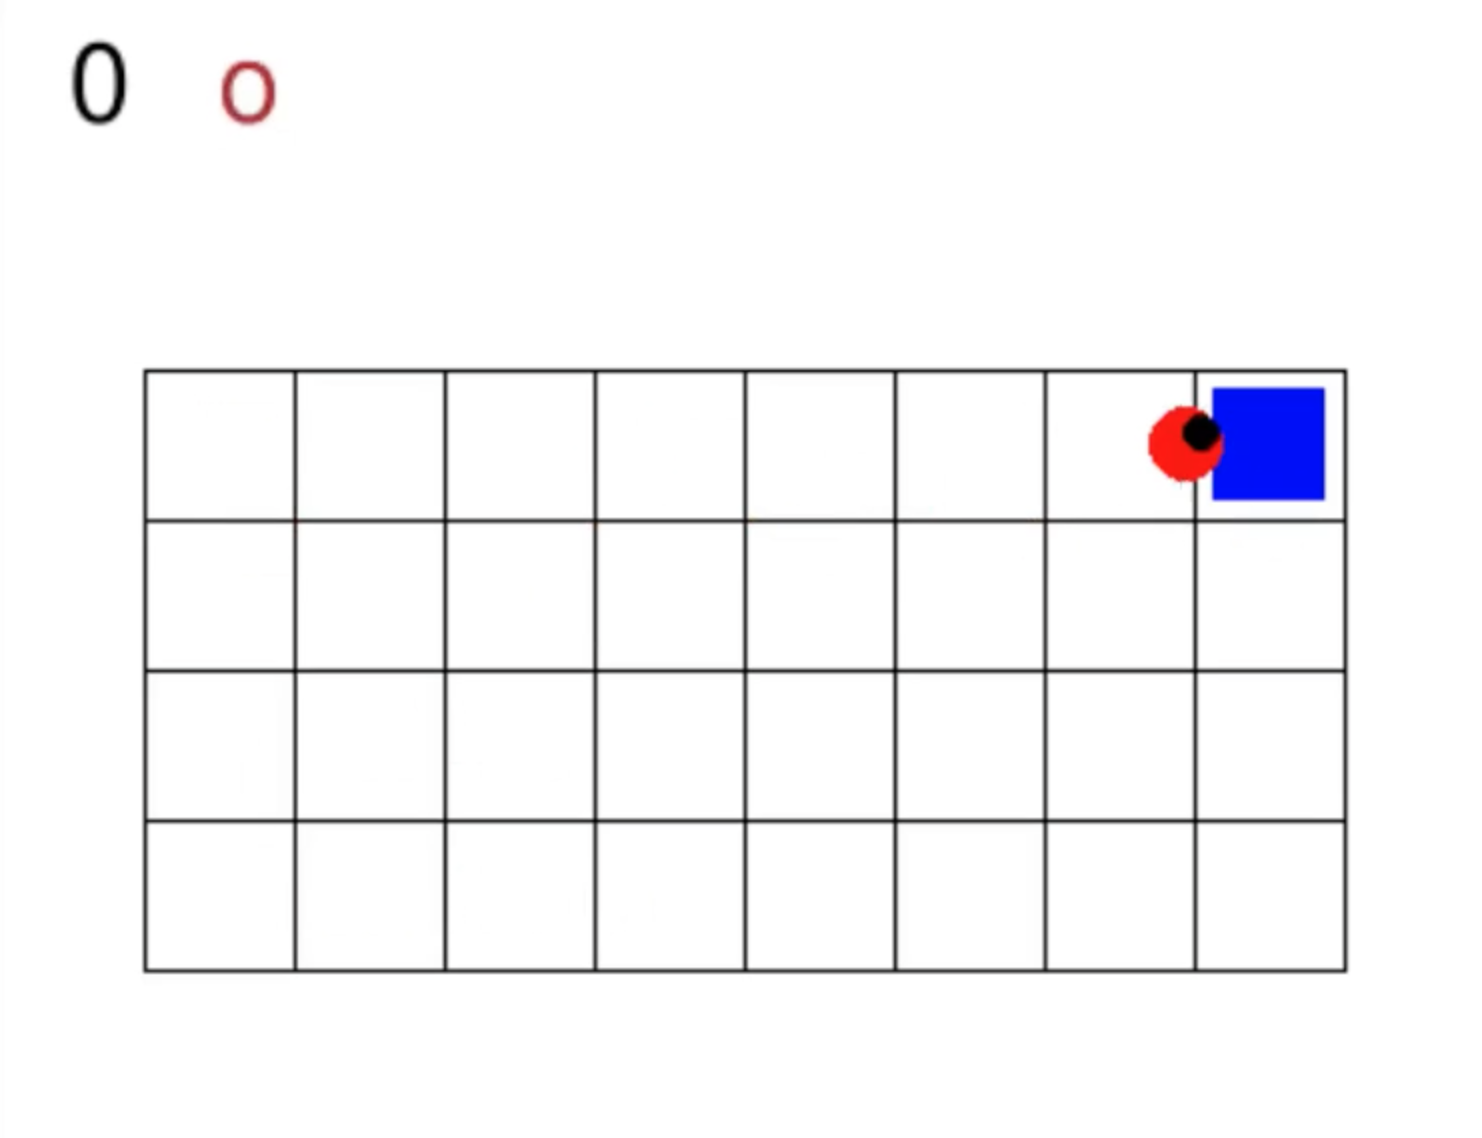
\includegraphics[width = 0.4\textwidth]{images/map1_easy.png}
    \caption{4x8 Gym Sapientino map for the experiment with one color. The initial position is in the cell [2,2].}
    \label{fig:m1e}
\end{figure}

\begin{table}[h!]
\centering
\begin{tabular}{|p{1cm}|p{2cm}|p{1cm}|p{1.2cm}|p{1.7cm}||}
 \hline
 \multicolumn{5}{|c|}{Agent hyperparameters} \\
 \hline
 Map & Algorithm & batch size & memory & exploration \\
 \hline
 easy & $DQN$ & 500 & 10000 & 0.5 \\
 \hline
 easy & $DQN_{CRM}$ & 500 & 10000 & 0.5 \\
\hline
\end{tabular}
\end{table}
\begin{table}[h!]
\centering
\begin{tabular}{||p{0.8cm}|p{1cm}|p{1.2cm}|p{1.7cm}| }
 \hline
 \multicolumn{4}{|c|}{Agent hyperparameters (contd.)} \\
    \hline
    lr & update frequency & episodes & timestamps\\
    \hline
    0.001 & 500 & 1000 & 500 \\
    \hline
    0.001 & 500 & 1000 & 500 \\
\hline
\end{tabular}
\caption{Table containing the relevant hyperparameter configuration of the tested agents related to the experiment with 1 color}\label{tab:t1e}
\end{table}
\begin{figure}[h!]
  \centering
  \subfloat[epoch-length]{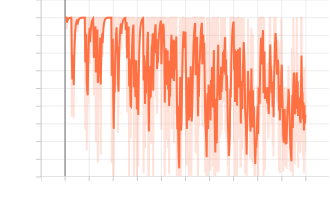
\includegraphics[width=0.4\textwidth]{images/length_1_easy.png}\label{fig:p1el}}
  \hfill
  \subfloat[epoch-reward]{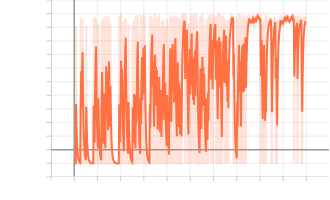
\includegraphics[width=0.4\textwidth]{images/reward_1_easy.png}\label{fig:p1er}}
  \caption{The training plots for  $DQN$ with parameters in Table \ref{tab:t1e}, in Sapientino Map with one colour in Figure \ref{fig:m1e}. The convergence rate increases as the epoch length decreases.}\label{fig:p1e}
\end{figure}
As shown in Table \ref{fig:p1e} the $DQN_{CRM}$ algorithm converges for the simple case of a single automata state. In the following experiments we performed the same experiment for a larger number of states.


\subsection{Two Colors Easy and Hard} %DONE

In this experiment we reproduced the same training but using two different maps to see how the presence of obstacles affect the training process.
Figure \ref{fig:m2h} shows the \textit{hard} case used in which there is an obstacle between the two temporal goals.

We can notice from plots in Figure \ref{fig:p2e} that the agent struggle at finding the first temporal goal, this is because the goal is particularly far from the initial position, the agent need to explore for several episodes before start getting some rewards.

\begin{figure}[h!]
  \centering
  \subfloat[Easy map with two colors]{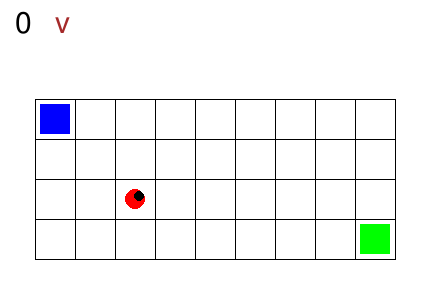
\includegraphics[width=0.4\textwidth]{images/sapientino.png}\label{fig:m2e}}
  \hfill
  \subfloat[Hard map with two colors]{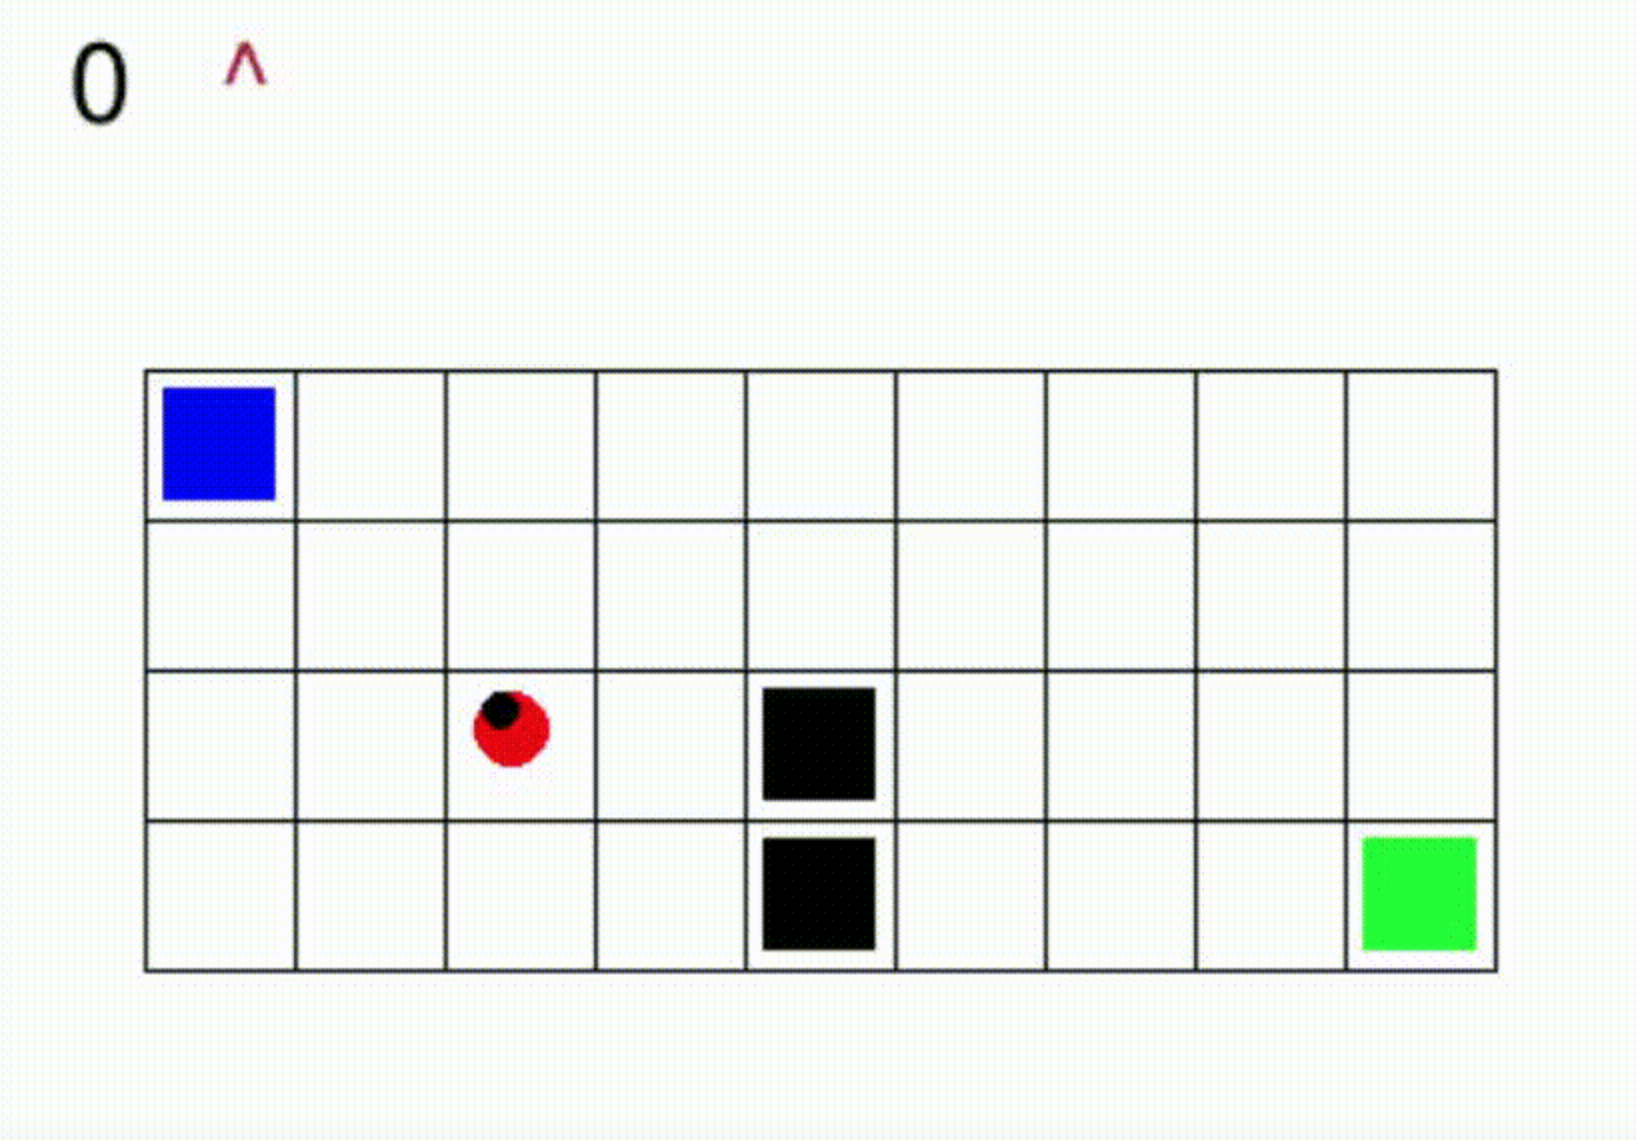
\includegraphics[width=0.4\textwidth]{images/map2_hard.png}\label{fig:m2h}}
  \caption{4x9 Gym Sapientino maps for the experiment with two color. The initial position is in the cell [2,2]. (b) shows the \textit{hard} case used in which there is an obstacle between the two temporal goals.}
\end{figure}
\begin{figure}[h!]
  \centering
  \subfloat[epoch-length]{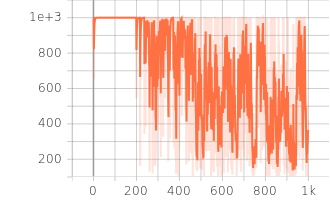
\includegraphics[width=0.4\textwidth]{images/length_2_easy.png}\label{fig:p2el}}
  \hfill
  \subfloat[epoch-reward]{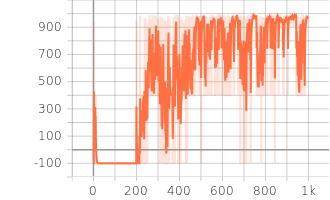
\includegraphics[width=0.4\textwidth]{images/reward_2_easy.png}\label{fig:p2er}}
  \caption{The training plots for DQN with parameters in Table \ref{tab:t2}, in an easy Sapientino Map with two colours in Figure \ref{fig:m2e}. The convergence rate increases as the epoch length decreases. }\label{fig:p2e}
\end{figure}
\begin{figure}[h!]
  \centering
  \subfloat[epoch-length]{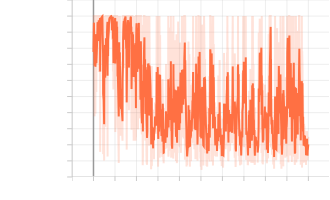
\includegraphics[width=0.4\textwidth]{images/length_2_hard.png}\label{fig:p2hl}}
  \hfill
  \subfloat[epoch-reward]{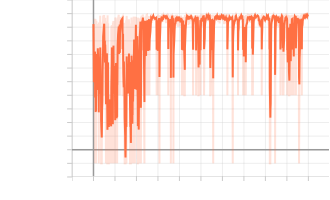
\includegraphics[width=0.4\textwidth]{images/reward_2_hard.png}\label{fig:p2hr}}
  \caption{The training plots for DQN with parameters in Table \ref{tab:t2}, in an \textit{hard} Sapientino Map with two colours in Figure \ref{fig:m2h}. Unexpectedly, using the parameters in Table \ref{tab:t2}, the training converges faster than the \textit{easy} case.
}
\end{figure}

\begin{table}[h]
    \centering
    \begin{tabular}{|p{1cm}|p{2cm}|p{1cm}|p{1.2cm}|p{1.7cm}||}
    \hline
    \multicolumn{5}{|c|}{Agent hyperparameters} \\
    \hline
    Map & Algorithm & batch size & memory & exploration \\
    \hline
    easy & DQN & 256 & 10000 & 0.4 \\
    \hline
    hard & DQN & 500 & 32500 & 0.5 \\
    \hline
    \end{tabular}
\end{table}

\begin{table}[h!]
\centering
\begin{tabular}{||p{0.8cm}|p{1cm}|p{1.2cm}|p{1.7cm}|}
 \hline
 \multicolumn{4}{|c|}{Agent hyperparameters (contd.)} \\
 \hline
lr & update frequency & episodes & timestamps\\
 \hline
 0.001 & 256 & 1000 & 500 \\
  \hline
  0.001 & 500 & 2000 & 1000 \\
\hline
\end{tabular}
\caption{Table containing the relevant hyperparameter configuration of the tested agents related to the experiment with 2 color}\label{tab:t2}
\end{table}

\subsection{Three Colors Easy and Hard} %DONE
In this experiment we tested again the convergence of the algorithm on harder maps with bigger obstacles. The Figure \ref{fig:m3h} shows a very hard map 6x11 in which there is a very large obstacle which separate two near temporal goals, in particular here the goal sequence is defined as \{\textit{blue},\textit{red},\textit{green}\}, which makes the problem really interesting since the agent has to perform very difficult maneuvers to reach each subgoal.\\
Looking at the plots in Figures \ref{fig:p3e} and \ref{fig:p3h}, it is easy to recognize how the presence of obstacles delays the learning and slow down the convergence.
\begin{figure}[h!]
  \centering
  \subfloat[Easy map with three colors]{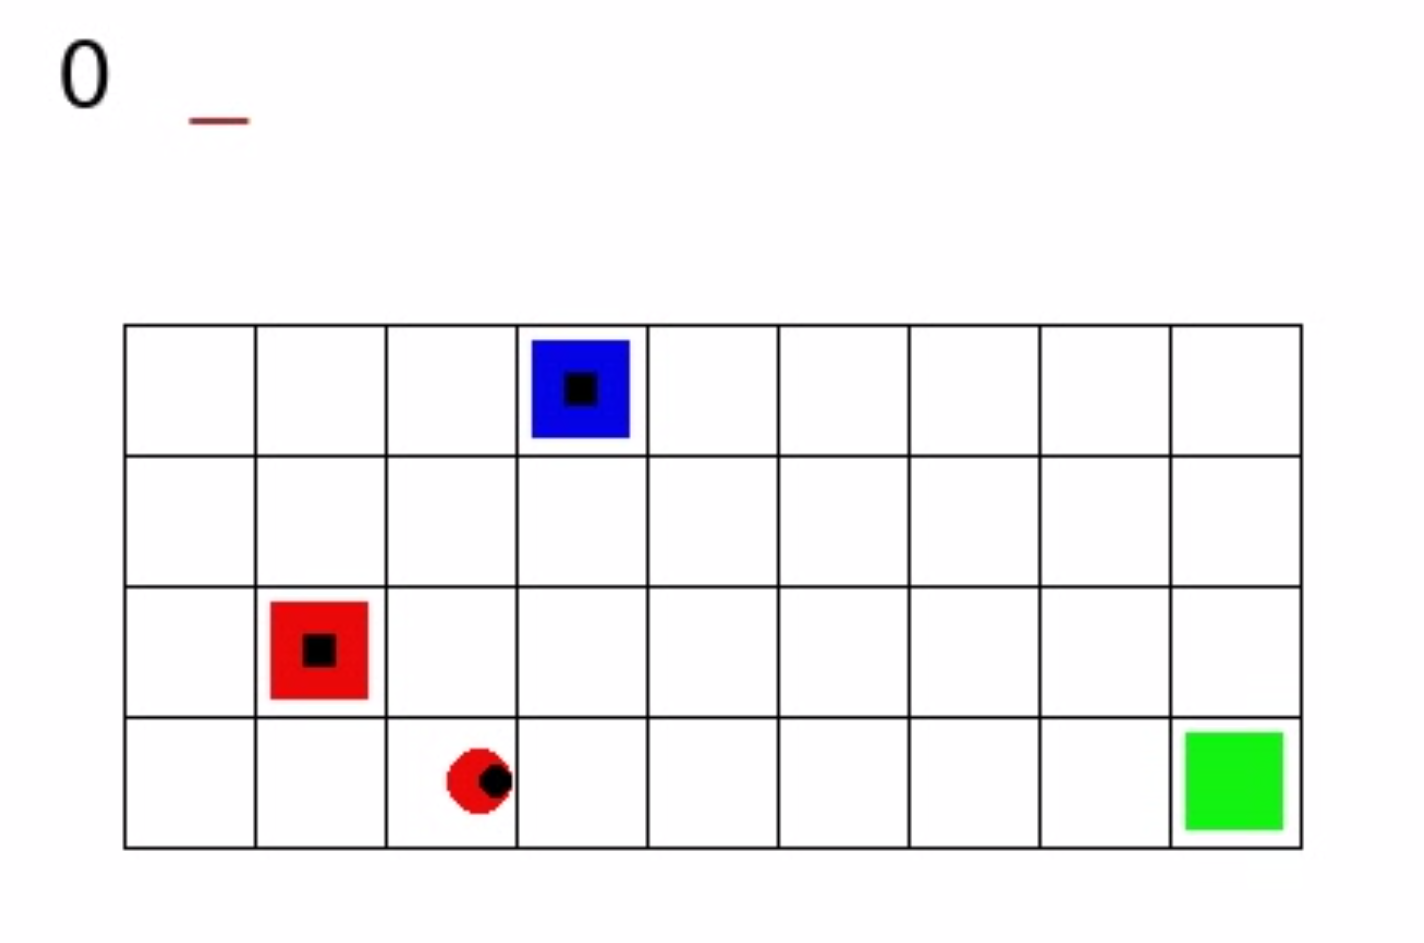
\includegraphics[width=0.4\textwidth]{images/map3_easy.png}\label{fig:m3e}}
  \hfill
  \subfloat[Hard map with three colors]{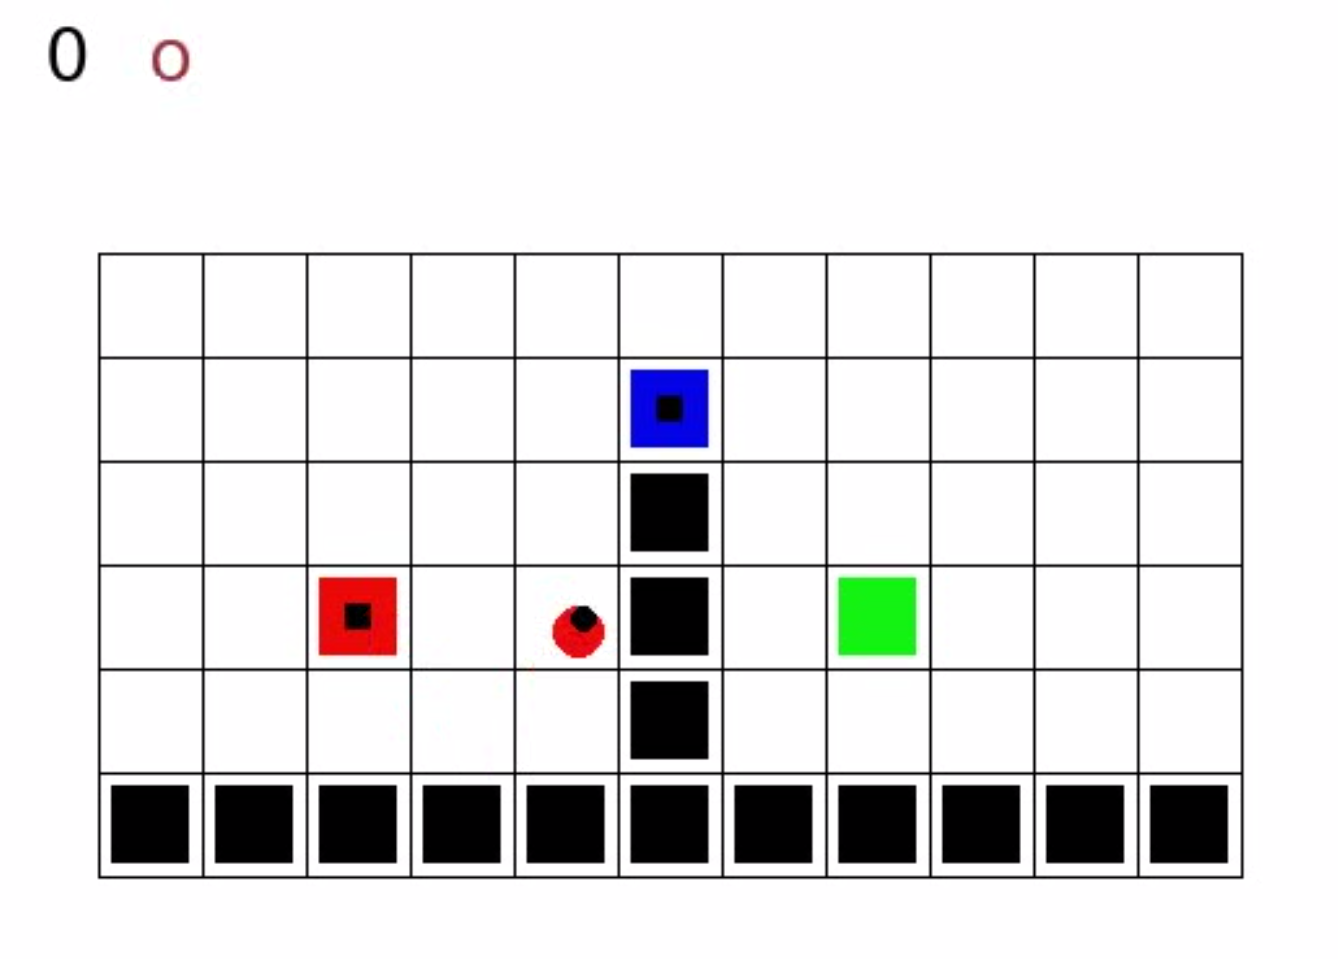
\includegraphics[width=0.4\textwidth]{images/map3_hard.png}\label{fig:m3h}}
  \caption{(a) 4x9 Gym Sapientino map for the easy experiment with three color. (b) 6x11 Gym Sapientino map shows the \textit{harder} map used in which there is an obstacle between the two temporal goals. The initial position is in the cell [2,2] for both experiments.}
\end{figure}
\begin{figure}[h!]
  \centering
  \subfloat[epoch-length]{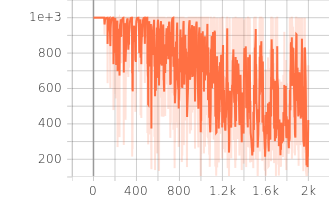
\includegraphics[width=0.4\textwidth]{images/length_3_easy.png}\label{fig:p3el}}
  \hfill
  \subfloat[epoch-reward]{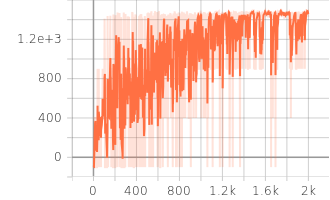
\includegraphics[width=0.4\textwidth]{images/reward_3_easy.png}\label{fig:p3er}}
  \caption{The training plots for DQN with parameters in Table \ref{tab:t3}, in an \textit{easy} Sapientino Map with three colours in Figure \ref{fig:m3e}.}\label{fig:p3e}
\end{figure}
\begin{figure}[h!]
  \centering
  \subfloat[epoch-length]{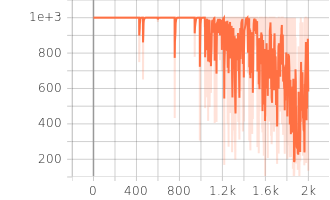
\includegraphics[width=0.4\textwidth]{images/length_3_hard.png}\label{fig:p3hl}}
  \hfill
  \subfloat[epoch-reward]{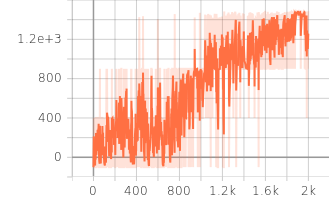
\includegraphics[width=0.4\textwidth]{images/reward_3_hard.png}\label{fig:p3hr}}
  \caption{The training plots for DQN with parameters in Table \ref{tab:t3}, in an \textit{hard} Sapientino Map with three colours in Figure \ref{fig:m3h}. The presence of obstacles delays the learning process with respect to the \textit{easy} case.}\label{fig:p3h}
\end{figure}
\begin{table}[h]
\centering
\begin{tabular}{|p{1cm}|p{2cm}|p{1cm}|p{1.2cm}|p{1.7cm}||}
 \hline
 \multicolumn{5}{|c|}{Agent hyperparameters} \\
 \hline
 Map & Algorithm & batch size & memory & exploration \\
 \hline
 easy & DQN & 32 & 10000 & 0.4 \\
  \hline
  hard & DQN & 500 & 32500 & 0.6 \\
\hline
\end{tabular}
\end{table}
\begin{table}[h!]
\centering
\begin{tabular}{||p{0.8cm}|p{1cm}|p{1.2cm}|p{1.7cm}|}
 \hline
 \multicolumn{4}{|c|}{Agent hyperparameters (contd.)} \\
 \hline
lr & update frequency & episodes & timestamps\\
 \hline
 0.001 & 32 & 2000 & 1000 \\
  \hline
  0.001 & 500 & 2000 & 1000 \\
\hline
\end{tabular}
\caption{Table containing the relevant hyperparameter configuration of the tested agents related to the experiment with 3 color}\label{tab:t3}
\end{table}


\subsection{Four Colors Easy} %DONE
In this experiment we used the color sequence \{\textit{blue},\textit{red},\textit{yellow},\textit{green}\}, Figure \ref{fig:m4c}. This sequence required a longer training with respect to the other experiments. In fact we can say the training time required is directly proportional to the number of colors, thus experts. \\
We performed this experiment using the DQN algorithm without CRM, the parameters used are shown in Table \ref{tab:t4}.
\begin{figure}[h!]
  \centering
  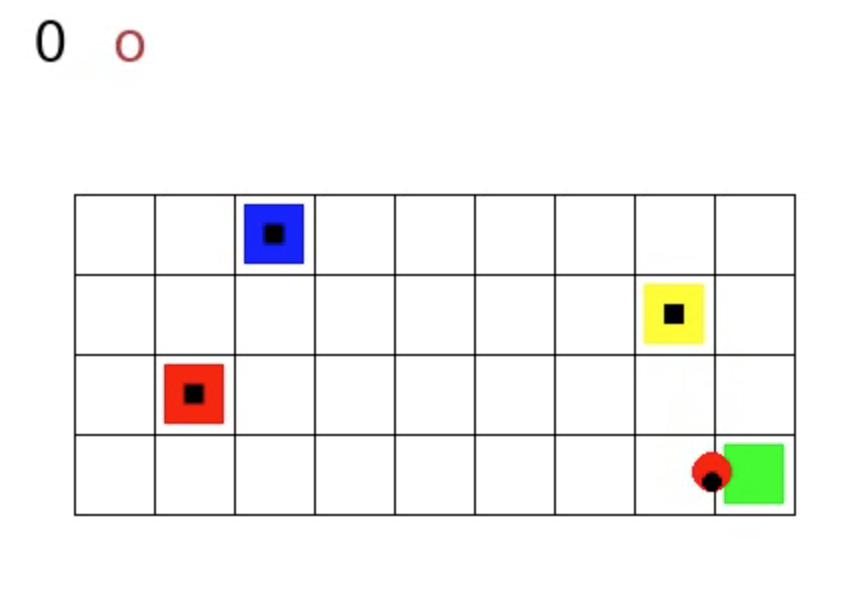
\includegraphics[width=0.4\textwidth]{images/map4_easy.png}
  \caption{The Sapientino Map we used for the experiment with 4 colours. The temporal goal sequence is \{\textit{blue},\textit{red},\textit{yellow},\textit{green}\}.}\label{fig:m4c}
\end{figure}
\begin{figure}[h!]
  \centering
  \subfloat[epoch-length]{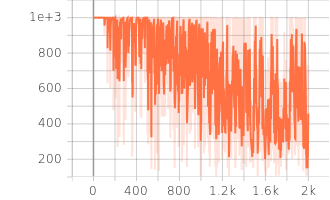
\includegraphics[width=0.4\textwidth]{images/length_4_easy.png}\label{fig:p4el}}
  \hfill
  \subfloat[epoch-reward]{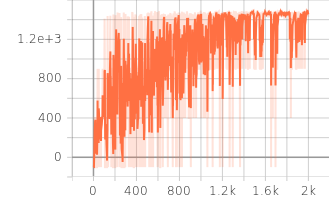
\includegraphics[width=0.4\textwidth]{images/reward_4_easy.png}\label{fig:p4er}}
  \caption{The training plots for DQN with parameters in Table \ref{tab:t4}, in Sapientino Map with four colours in Figure \ref{fig:m4c}. The convergence rate increases as the epoch length decreases. }\label{fig:p4}
\end{figure}
\begin{table}[h]
\centering
\begin{tabular}{|p{1cm}|p{2cm}|p{1cm}|p{1.2cm}|p{1.7cm}||}
 \hline
 \multicolumn{5}{|c|}{Agent hyperparameters} \\
 \hline
 Map & Algorithm & batch size & memory & exploration \\
 \hline
 4 easy & DQN & 500 & 32500 & 0.5 \\
\hline
\end{tabular}
\end{table}
\begin{table}[h!]
\centering
\begin{tabular}{||p{0.8cm}|p{1cm}|p{1.2cm}|p{1.7cm}| }
 \hline
 \multicolumn{4}{|c|}{Agent hyperparameters (contd.)} \\
 \hline
lr & update frequency & episodes & timestamps\\
 \hline
 0.001 & 500 & 2000 & 1000 \\
\hline
\end{tabular}
\caption{Table containing the relevant hyperparameter configuration of the tested agents related to the experiment with 4 colours.}\label{tab:t4}
\end{table}
From the plots in Figure \ref{fig:p4} we can understand how the agent learns to converge faster as the episodes increase. Anyway convergence is reached at half epochs, but the epochs left are needed to optimize the time for convergence.

\section{Conclusion and result discussion} %DONE, BUT CAN BE EXPANDED

In this paper we have proposed a Tensorforce based non markovian agent implementation which is able to solve a non markovian navigation task in \textit{Gym Sapientino}.
We proved the effectiveness of the method, showing that it is possible to solve temporal goals in this domain by using as many specialized experts in the hidden layers as the automata states.\\
We used \textit{Reward Shaping} which has been shown from\footnote{\url{https://github.com/francycar/RA_project}} to have many benefits, they also shown that the sparse reward problem, which was one of the major issue our agent experienced in the training process, can be easily overcome by introducing intermediate positive rewards which boost the learning process and encourages the agent to complete the various steps that are needed to reach the goal in  a supervised manner.\\
We realized an implementation of the \textit{Counterfactual Experiences for Reward Machines} algorithm (Section \ref{sec:CRM}) in \textit{Tensorforce} framework by customizing the \textit{Sapientino Case} environment to separate the \textit{Deterministic Finite Automata} (Section \ref{sec:dfa}) from the \texttt{gym.Environment} in order to cycle over the automata states as described in Equation \ref{eq:crm}. Moreover we conduct several experiments to demonstrate the success of the implementation and of the CRM algorithm itself. In particular we noticed, but it is also intuitive a priori, that the CRM algorithm is particularly useful when dealing with larger automata state spaces. On the counter part it is particularly time consuming when implemented to run locally on the CPU, especially for larger state spaces.

\newpage

\bibliography{main}
\bibliographystyle{plain}

\end{document}
